\documentclass[10pt,reqno]{book}
\usepackage{amsmath,amssymb,amsfonts,amsthm}
\usepackage{graphics,tikz,caption}
\usepackage{emptypage}
\usepackage{pgfplots}
\usepackage{algorithm}
\usepackage[noend]{algpseudocode}
\usepackage{listings}
\usepackage{booktabs}
\usepackage{graphicx}
\usepackage{ mathrsfs }
\usepackage{bm}
\usepackage{tikz-3dplot}
\usepackage{bigints}
\usetikzlibrary{patterns}
\usetikzlibrary{3d}
\graphicspath{ {images/} }
\usetikzlibrary{decorations.pathmorphing,patterns}
\pgfplotsset{compat=1.8}


\DeclareGraphicsExtensions{.pdf}
\parindent 1cm
\parskip 0.2cm
\topmargin 0.2cm
\oddsidemargin 1cm
\evensidemargin 0.5cm
\textwidth 15cm
\textheight 21cm
\theoremstyle{definition}
\newtheorem{theorem}{Theorem}[section]
\newtheorem{proposition}[theorem]{Proposition}
\newtheorem{corollary}[theorem]{Corollary}
\newtheorem{lemma}[theorem]{Lemma}
\newtheorem{remark}[theorem]{Remark}
\newtheorem{definition}[theorem]{Definition}
\newtheorem{example}{Example}




\newcommand{\ihat}{\boldsymbol{\hat{\imath}}}
\newcommand{\jhat}{\boldsymbol{\hat{\jmath}}}
\newcommand{\khat}{\boldsymbol{\hat{\kmath}}}

\def\L{\mathscr{L}}
\def\R{\mathbb{R}}
\def\S{\mathbb{S}}
\def\I{\mathbb{I}}
\makeindex

\font\myfont=cmr12 at 20pt

\title{\myfont{Calculus II}}

\author{Lukas Zamora}

\date{December 2, 2017}
\pagestyle{headings}
\pagenumbering{roman}



\begin{document}
	
	\maketitle
	\addcontentsline{toc}{chapter}{Contents}
	\pagenumbering{arabic}
	
	\tableofcontents
	
	
	\chapter{Integration Techniques}
	
	
	\section{Integration by Parts}
	
	In this section we look at integrals of the form
	\[ \int f(x)\,g(x)\,dx \]
	Usually we can get by with a simple $ u $-substitution. But in most cases it wont work for more complex integrals. So we use a technique called \textit{integration by parts}. Lets start with the product rule.
	\[ (fg)' = f'g + fg' \]
	Now, integrate both sides of this.
	\[ \int (fg)'\,dx = \int f'g + fg'\,dx \]
	The left side is easy enough to integrate and we'll split up the right side of the integral using properties of integrals.
	\[ fg = \int f'g\,dx + \int fg'\,dx \]
	Note that technically we should have had a constant of integration show up on the left side after doing the integration. We can drop it at this point since other constants of integration will be showing up down the road and they would just end up absorbing this one. Finally, rewrite the formula as follows and we arrive at the integration by parts formula.
	\[ \int fg'\,dx = fg - \int f'g\,dx \]
	This is not the easiest formula to use however. So, let's do a couple of substitutions.
	\begin{center}
		\begin{tabular}{cc}
			$ u = f(x) $    &    $ v = g(x) $    \\
			$ du = f'(x)\,dx $ & $ dv = g'(x)\,dx $
		\end{tabular}	
	\end{center}
	Using these substitutions gives us the formula that most people think of as the integration by parts formula.
	\[ \int u\,dv = uv - \int v\,du \]
	Next, let's take a look at integration by parts for definite integrals. The integration by parts formula for definite integrals is,
	\[ \int\limits_{a}^{b} u\,dv = uv\Big|_{a}^{b} - \int\limits_{a}^b v\,du \]
	
	\section{Trigonometric Substitutions}
	
	Let's take a look at the following integral.
	\[ \int \frac{\sqrt{25x^2 - 4}}{x}\,dx \]
	In this case the substitution $ u = 25x^2-4 $ will not work and so we're going to have to do something different for this integral. It would be nice if we could get rid of the square root somehow. The following substitution will do that for us.
	\[ x = \frac{2}{5}\sec(\theta) \]
	Before we actually do the substitution however let's verify the claim that this will allow us to get rid of the square root.
	\[ \sqrt{25x^2-4} = \sqrt{25\left(\dfrac{4}{25}\right)\sec^2(\theta)-4} = \sqrt{4(\sec^2(\theta)-1)} = \sqrt{4\tan^2(\theta)} = 2\tan(\theta) \]
	So, we were able to eliminate the square root using this substitution. Let's now do the substitution and see what we get. In doing the substitution don't forget that we'll also need to substitute for the $ dx $. This is easy enough to get from the substitution.
	\[ x = \frac{2}{5}\sec(\theta) \qquad \Rightarrow \qquad dx = \frac{2}{5}\sec(\theta)\tan(\theta)\,d\theta \]
	Using this substitution the integral becomes,
	\begin{align*}
		\int \frac{\sqrt{25x^2 - 4}}{x}\,dx &= \int \frac{2\tan(\theta)}{\frac{2}{5}\sec(\theta)}\left(\frac{2}{5}\sec(\theta)\tan(\theta)\right) d\theta\\
		&= 2 \int \tan^2(\theta)\,d\theta\\
		&= 2\int \sec^2(\theta) - 1\,d\theta\\
		&= 2(\tan(\theta) - \theta) +C
	\end{align*}
	So, we've got an answer for the integral. Unfortunately the answer isn't given in $ x $'s as it should be. So, we need to write our answer in terms of $ x $. We can do this with some right triangle trig. From our original substitution we have the following right triangle,
	\begin{center}
		\begin{tikzpicture}
			\draw (0,0) -- (4,0);
			\draw (4,0) -- (4,2);
			\draw (0,0) -- (4,2);
			\node[below=1mm] at (2,0) {$2$};
			\node[above=1mm] at (2,1) {$5x$};
			\node[right] at (4,1) {$\sqrt{25x^2-4}$};
			\node at (1,0.25) {$\theta$};
		\end{tikzpicture}
	\end{center}
	From this we can see that,
	\[ \tan(\theta) = \frac{\sqrt{25x^2-4}}{2} \]
	We can deal with the $ \theta $ in one of any variety of ways. From our substitution we can see that,
	\[ \theta = \cos^{-1}\left(\frac{2}{5x}\right) \]
	So, with all of this the integral becomes,
	\begin{align*}
		\int \frac{\sqrt{25x^2 - 4}}{x}\,dx &= 2\left( \frac{\sqrt{25x^2-4}}{2} - \cos^{-1}\left(\frac{2}{5x}\right) \right) + C\\
		&=  \sqrt{25x^2-4} - 2\cos^{-1}\left(\frac{2}{5x}\right) + C
	\end{align*}
	We now have the answer back in terms of $ x $.\\ \\
	Before leaving this section let's summarize all three cases in one place.
	\begin{center}
		\begin{tabular}{ccc}
			$ \sqrt{a^2-b^2x^2} $ & $ \Rightarrow $ & $ x = \dfrac{a}{b}\sin(\theta) $ \\ \\
			$ \sqrt{b^2x^2-a^2} $ & $ \Rightarrow $ & $ x = \dfrac{a}{b}\sec(\theta) $ \\ \\ 
			$ \sqrt{a^2+b^2x^2} $ & $ \Rightarrow $ & $ x = \dfrac{a}{b}\tan(\theta) $ \\
		\end{tabular}	
	\end{center}

	\section{Partial Fractions}
	
	In this section we look at integrating rational expressions of polynomials. Mainly expressions we can't integrate with just a simple $ u $-substitution, like this integral for example
	\[ \int \frac{3x + 11}{x^2 - x -6}\,dx \]
	However, we notice that the integrand can be broken up as follows,
	\[ \frac{3x + 11}{x^2 - x - 6} = \frac{4}{x - 3} - \frac{1}{x + 2} \]
	then the integral is quite simple,
	\begin{align*}
		\int \frac{3x + 11}{x^2 - x -6}\,dx &= \int \frac{4}{x - 3} - \frac{1}{x + 2}\,dx\\
		&= 4\ln|x-3| - \ln|x+2| + C
	\end{align*}	
	This process of taking a rational expression and decomposing it into simpler rational expressions that we can add or subtract to get the original expression is called \textit{partial fraction decomposition}. Many integrals involving rational expressions can be done if we first do partial fractions on the integrand.\\ \\
	So let's review on partial fractions. We'll start with a rational expression in the form
	\[ f(x) = \frac{P(x)}{Q(x)} \]
	where both $ P(x) $ and $ Q(x) $ are polynomials and the degree of $ P(x) $ is smaller than the degree of $ Q(x) $. Partial fractions can only be done in this form, so it's important to remember that.\\ \\
	So, once we've determined that partial fractions can be done we factor the denominator as completely as possible. Then for each factor in the denominator we can use the following table to determine the term(s) we pick up in the partial fraction decomposition.
	
	\begin{center}
		\begin{tabular}{c|c}
			Factor in denominator & Term in partial fraction decomposition\\ \hline
			$ ax+b $ & $ \dfrac{A}{ax+b} $ \\ [2ex] 
			$ ax^2 + bx + c $ & $ \dfrac{Ax + B}{ax^2 + bx + c} $\\ [2ex] 
			$ (ax+b)^n $ & $ \dfrac{A_1}{ax+b} + \dfrac{A_2}{(ax+b)^2} + \ldots + \dfrac{A_n}{(ax+b)^n} $, $ n = 1,2,3,\ldots $\\ [2ex]
			$ (ax^2 + bx + c)^n $ & $ \dfrac{A_1x + B_1}{ax^2+bx+c} + \dfrac{A_2x + B_2}{(ax^2+bx+c)^2} + \ldots + \dfrac{A_nx + B_n}{(ax^2+bx+c)^n} $, $ n=1,2,3,\ldots $
		\end{tabular}
	\end{center}
	Now, let's redo the example using the table above. Factoring the denominator we get,
	\[ \frac{3x + 11}{(x-3)(x+2)} = \frac{A}{x-3} + \frac{B}{x+2} \]
	Now all we need to is find our $ A $ and $ B $,
	\begin{align*}
		\frac{3x + 11}{(x-3)(x+2)} &= \frac{A}{x-3} + \frac{B}{x+2}\\
		\frac{3x + 11}{(x-3)(x+2)} &= \frac{A(x+2) + B(x-3)}{(x-3)(x+2)}\\
		3x + 11 &= A(x+2) + B(x-3)\\
		3x + 11 &= Ax + 2A + Bx - 3B
	\end{align*}
	Now we have a $ 2\times 2 $ system of equations to solve.
	\begin{equation*}
		\begin{cases}
			3 = A + B\\
			11 = 2A - 3B
		\end{cases}
	\end{equation*}
	Solving this gives us $ A = 4 $ and $ B = -1 $, so our integral now becomes
	\begin{align*}
		\int \frac{3x + 11}{(x-3)(x+2)}\,dx &= \int \frac{4}{x-3} - \frac{1}{x+2}\,dx\\
		&= 4\ln|x-3| - \ln|x+2| +C                                          	
	\end{align*}

	\section{Improper Integrals}
	
	In this section we deal with a special type of integral that will appear a lot in more upper-level courses. These are called \textit{improper integrals}. Let's start with the first kind.\\ \\
	\textbf{Infinite Interval}\\
	In this kind of integral one or both of the limits of integration are infinity. In these cases the interval of integration is said to be over an infinite interval. Here is an example 
	\[ \int_{1}^{\infty} \frac{1}{x^2}\,dx \]
	To do this we simply take a limit of another variable, but switching the infinity and our new variable in the limit of integration. 
	\begin{align*}
		\int_{1}^{\infty} \frac{1}{x^2}\,dx &= \lim\limits_{t \to \infty} \int_{1}^{t} \frac{1}{x^2}\,dx\\
		&= \lim\limits_{t \to \infty} \left( -\frac{1}{x} \right) \Bigg|_{1}^{t}\\
		&= \lim\limits_{t \to \infty} \left( 1 - \frac{1}{t} \right) = 1
	\end{align*}
	We call these integrals \textit{convergent} if the associated limit exists and is a finite number and \textit{divergent} if the associated limit either doesn't exist or converges to plus/minus infinity.\\ \\
	There are essentially three cases that these integrals fall into.
	\begin{enumerate}
		\item If $ \int_{a}^{t} f(x)\,dx $ exists for every $ t > a $ then,
			\[ \int_{a}^{\infty} f(x)\,dx = \lim\limits_{t \to \infty} \int_{a}^{t} f(x)\,dx \]
			provided the limit exists and is finite.
			
		\item If $ \int_{t}^{b} f(x)\,dx $ exists for every $ t < b $ then,
			\[ \int_{-\infty}^{b} f(x)\,dx = \lim\limits_{t \to -\infty} \int_{t}^{b} f(x)\,dx \]
			provided the limit exists and is finite.
			
		\item If $ \int_{-\infty}^{c} f(x)\,dx $ and $ \int_{c}^{\infty} f(x)\,dx $ are both convergent then,
			\[ \int_{-\infty}^{\infty} f(x)\,dx = \int_{-\infty}^{c} f(x)\,dx + \int_{c}^{\infty} f(x)\,dx \]
			where $ c $ is any number. Note that this requires \textbf{both} of the integrals to be convergent in order for the integral to also be convergent. If either of the two integrals is divergent then so is this integral.
 	\end{enumerate}
 
 	\noindent \textbf{Discontinuous Integrand}\\
 	We now need to look at the second type of improper integrals that we'll be looking at in this section. These are integrals that have discontinuous integrands. The process here is basically the same with one subtle difference. Here are the general cases that we'll look at for these integrals.
 	\begin{enumerate}
 		\item If $ f(x) $ is continuous on the interval $ [a,b] $ and not continuous at $ x = b $ then,
 			\[ \int_a^b f(x)\,dx = \lim\limits_{t \to b^-} \int_a^t f(x)\,dx \]
 			provided the limit exists and is finite. Note as well that we do need to use a left hand limit here since the interval of integration is entirely on the left side of the upper limit.
 			
 		\item If $ f(x) $ is continuous on the interval $ [a,b] $ and not continuous at $ x = a $ then,
 			\[ \int_a^b f(x)\,dx = \lim\limits_{t \to a^+} \int_t^b f(x)\,dx \]
 			provided the limit exists and is finite. Note as well that we do need to use a right hand limit here since the interval of integration is entirely on the right side of the lower limit.
 		
 		\item If $ f(x) $ is not continuous at $ x = c $ where $ a < c < b $ and $ \int_a^c f(x)\,dx $ and $ \int_c^b f(x)\,dx $ are both convergent then,
 			\[ \int_a^b f(x)\,dx = \int_a^c f(x)\,dx + \int_c^b f(x)\,dx \]
 			As with the infinite interval case this requires \textbf{both} of the integrals to be convergent in order for this integral to also be convergent.
 			
 		\item If $ f(x) $ is not continuous at $ x = a $ and $ x = b $ and if $ \int_a^c f(x)\,dx $ and $ \int_c^b f(x)\,dx $ are both convergent then,
 		\[ \int_a^b f(x)\,dx = \int_a^c f(x)\,dx + \int_c^b f(x)\,dx \]
 		Where $ c $ is any number. Again, this requires \textbf{both} of the integrals to be convergent in order for this integral to also be convergent.
 	\end{enumerate}
 	Note that the limits in these cases really do need to be right or left hand limits. Since we will be working inside the interval of integration we will need to make sure that we stay inside that interval. This means that we'll use one-sided limits to make sure we stay inside the interval.\\ \\
 	\textbf{Example}
 	\[ \int_0^3 \frac{1}{\sqrt{3-x}}\,dx \]
	The problem is the upper limit so we are in the first case above.
	\begin{align*}
		\int_0^3 \frac{1}{\sqrt{3-x}}\,dx &= \lim\limits_{t \to 3^-} \int_0^t \frac{1}{\sqrt{3-x}}\,dx\\
		&= \lim\limits_{t \to 3^-} (-2\sqrt{3-x})\Big|_0^t\\
		&= \lim\limits_{t \to 3^-} (2\sqrt{3} - 2\sqrt{3-t}) = 2\sqrt{3}
	\end{align*}
	The limit exists and is finite so the integral converges and the integral's value is $ 2\sqrt{3} $.

	\chapter{Applications of Integrals}
	
	In this chapter we will look at some applications of integration. It should be noted as well that these applications are presented here, as opposed in Calculus I, simply because many of the integrals that arise from these applications tend to require techniques from the previous chapter.
	
	\section{Arc Length}
	
	In this section we want to determine the length of a continuous function $ y = f(x) $ on the interval $ [a,b] $. We'll also need to assume that the derivative is continuous on $ [a,b] $.\\ \\
	Initially we'll need to estimate the length of the curve. We'll do this by dividing the interval up into $ n $ equal subintervals each of width $ \Delta x $ and we'll denote the point on the curve at each point by $ Q_i $. We can then approximate the curve by a series of straight lines connecting the points.
	\begin{center}
		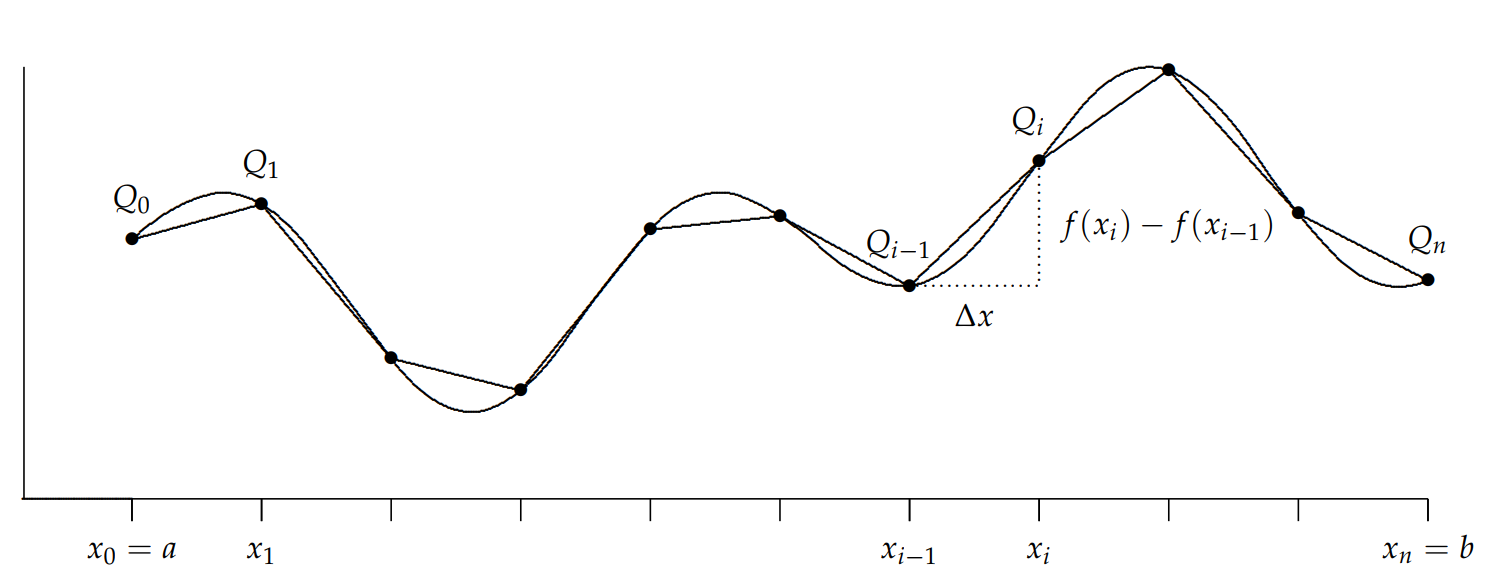
\includegraphics[scale=0.325]{arc.png}
	\end{center}
	Now denote the length of each of these segments by $ \big| Q_{i-1} Q_i \big| $ and the length of the curve will then be approximately 
	\[ L \approx \sum\limits_{i=1}^{n} \big| Q_{i-1} Q_i \big| \]
	and to get an exact length we can make $ n $ larger and larger. In other words,
	\[ L = \lim\limits_{n \to \infty} \sum\limits_{i=1}^{n} \big| Q_{i-1} Q_i \big| \]
	On each segment let's define $ \Delta y = f(x_i) - f(x_{i-1}) $. We can then compute directly the length of the line segments as follows
	\[ \big| Q_{i-1} Q_i \big| = \sqrt{(x_i - x_{i-1})^2 + (y_i - y_{i-1})^2} = \sqrt{\Delta x^2 + \Delta y_i^2} \]
	By the Mean Value Theorem we know that on the interval $ [x_{i-1},x_i] $ there is a point $ x_i^* $ such that,
	\[ f(x_i) - f(x_{i-1}) = f'(x_i^*)(x-x_{i-1}) \]
	\[ \Delta y_i = f'(x_i^*) \Delta x \]
	Therefore, the length can now be written as,
	\begin{align*}
		\big| Q_{i-1} Q_i \big| &= \sqrt{ \Delta x^2 + [f'(x_i^*)]^2 \Delta x^2}\\
		&= \sqrt{1 + [f'(x_i^*)]^2} \, \Delta x
	\end{align*}		
	The exact length of the curve is then 
	\[ L = \lim\limits_{n \to \infty} \sqrt{1 + [f'(x_i^*)]^2} \, \Delta x \]
	However, using the definition of the definite integral, this is nothing more than,
	\[ L = \int_a^b \sqrt{1 + [f'(x)]^2}\,dx \]
	A slightly more convenient notation is the following 
	\[ L = \int_a^b \sqrt{1 + \left( \frac{dy}{dx} \right)^2}\,dx \]
	In a similar fashion we can also derive a formula for $ x = h(y) $ on $ [c,d] $. 
	\[ L = \int_c^d \sqrt{1 + \left( \frac{dx}{dy} \right)^2}\,dy \]
	If we were to zoom in on the function, we could get a picture similar to this, where $ ds $ is a little distance of the function
	
	\begin{center}
		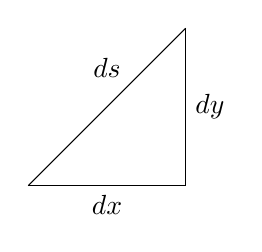
\begin{tikzpicture}
			\draw(0,0) -- (2,0);
			\draw(2,0) -- (2,2);
			\draw(0,0) -- (2,2);
			\draw(1,0) node[below] {$dx$};
			\draw(1,1.25) node[above] {$ds$};
			\draw(2,1) node[right] {$dy$};
		\end{tikzpicture}
	\end{center}
	
	\noindent Using the Pythagorean Theorem, we find that $ ds = \sqrt{dx^2 + dy^2} $. Knowing that $ L = \int ds $, we can substitute $ ds $ in 
	\begin{align*}
		L &= \int ds\\
		&= \int \sqrt{dx^2 + dy^2}\\
		&= \int \sqrt{1 + \left( \frac{dy}{dx} \right)^2}\,dx
	\end{align*}
	So there is a couple of ways to approach this.
	
	
	\section{Center of Mass}
	
	In this section we are going to find the \textit{center of mass} or \textit{centroid} of a thin plate with uniform density $ \rho $. The center of mass or centroid of a region is the point in which the region will be perfectly balanced horizontally if suspended from that point.\\ \\
	So, let's suppose that the plate is the region bounded by the two curves $ f(x) $ and $ g(x) $ on the interval $ [a,b] $. So, we want to find the center of mass of the region below.
	\begin{center}
		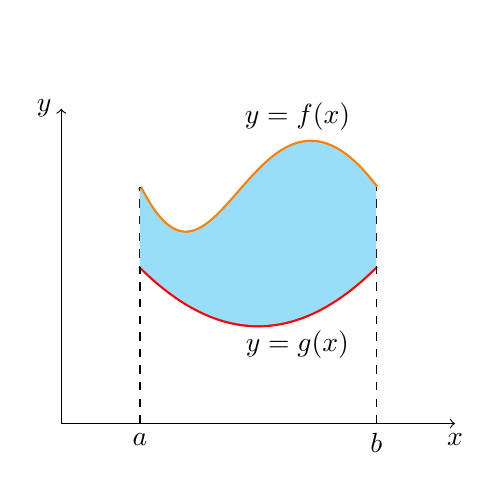
\begin{tikzpicture}
		% Axis
		\draw[->] (0,-1) -- (5,-1) node[below] {$x$};
		\draw[->] (0,-1) -- (0,3) node[left] {$y$};
		
		% Curves
		\draw[ultra thick,draw=orange] (1,2) .. controls (2,0) and (2.5,4) .. (4,2);
		\draw[ultra thick,draw=red] (1,1) .. controls (2,0) and (3,0) .. (4,1);
		\draw[dashed] (1,-1) -- (1,2);
		\draw[dashed] (4,-1) -- (4,2);
		
		% Area
		\path[fill=cyan!40] (1,1) -- (1,2) -- (1,2) .. controls (2,0) and (2.5,4) .. (4,2) -- (4,1) -- (4,1) -- (1,1) .. controls (2,0) and (3,0) .. (4,1);
		
		% Nodes
		\draw(1,-1) node[below] {$a$};
		\draw(4,-1) node[below] {$b$};
		\draw (3,0) node {$y=g(x)$};
		\draw (3,2) node[above=6mm] {$y=f(x)$};
		\end{tikzpicture}
	\end{center}
	We first need to find the mass of this plate. The mass is
	\begin{align*}
		m &= \rho(\text{Area of plate})\\
		  &= \rho \int_a^b f(x) - g(x)\,dx 
	\end{align*}		
	Next we'll need to find the \textit{moments} of the region. There are two moments, denoted by $ M_x $ and $ M_y $. The moments measure the tendency of the region to rotate about the $ x $ and $ y $-axis respectively. The moments are given by
	\begin{align*}
		M_x &= \rho \int_a^b \frac{1}{2} \left( [f(x)]^2 - [g(x)]^2 \right)\,dx\\
		M_y &= \rho \int_a^b x (f(x) - g(x))\,dx
	\end{align*}
	The coordinates of the center of mass, $ (\bar{x},\bar{y}) $, are then
	\begin{align*}
		\bar{x} &= \frac{M_y}{m}\\
		\bar{y} &= \frac{M_x}{m}
	\end{align*}
	
	\chapter{Parametric Equations and Polar Coordinates}
	
	\section{Parametric Equations and Curves}
	
	To this point we've looked almost exclusively at functions in the form $ y = f(x) $ or $ x = h(y) $ and almost of the formulas that we've developed require that functions be in one of these two forms. The problem is that not all curves or equations that we will look at fall easily into this form.\\ \\
	Take, for example, a circle. It is easy enough to write down the equation of a circle centered at the origin with radius $ r $.
	\[ x^2 + y^2 = r^2 \]
	However, we will never be able to write down the equation of a circle down as a single equation in either of the forms above. Sure we can solve for $ x $ or $ y $ as the following formulas show
	\[ y = \pm \sqrt{r^2 - x^2} \qquad x = \pm \sqrt{r^2 - y^2} \]
	but there are in fact two functions in each of these. Each formula gives a portion of the circle
	
	\begin{center}
		\begin{tabular}{ll}
			$ y = \sqrt{r^2 - x^2} $ (top) & $ x = \sqrt{r^2 - x^2} $ (right side) \\[3ex]
			$ y = -\sqrt{r^2 - x^2} $ (bottom) & $ x = -\sqrt{r^2 - x^2} $ (left side)
		\end{tabular}
	\end{center}
	Unfortunately we usually are working on the whole circle, or simply ca't say that we're going to be working only on one portion of it. Even if we can narrow things down to only one of these portions the function is still often fairly unpleasant to work with.\\ \\
	There are also many curves out there that we can't even write down as a single equation in terms of only $ x $ and $ y $. So, to deal with some of these problems we introduce \textit{parametric equations}. Instead of defining $ y $ in terms of $ x $ or vice versa, we define both $ x $ and $ y $ in terms of a third variable called a parameter.
	\[ x = f(t) \qquad y = g(t) \]
	This third variable is usually denoted by $ t $. Sometimes we will restrict the values of $ t $ that we'll use and at other times we won't.\\ \\
	Each value of $ t $ defines a point $ (x,y) = (f(t),g(t) $ that we can plot. The collection of points that we get by letting $ t $ be all possible values is the graph of the parametric equations and is called the \textit{parametric curve}.
	
	\section{Tangents with Parametric Equations}
	
	In this section we want to find the tangent lines to the parametric equations given by,
	\[ x = f(t) \qquad y = g(t) \]
	To do this let's first recall how to find the tangent line to $ y = \psi(x) $ at $ x = a $. Here the tangent line is given by,
	\[ y = \psi(a) + m(x-a) \]
	where $ m = \psi'(a) $. Now, notice that if we could figure out how to get the derivative $ \dfrac{dy}{dx} $ from the parametric equations we could simply reuse this formula since we will be able to use the parametric equations to find the $ x $ and $ y $ coordinates of the point.\\ \\
	So, just for a second let's suppose that we are able to eliminate the parameter from the parametric form and write the parametric equations in the form $ y = \psi(x) $. Now, plug the parametric equations in for $ x $ and $ y $. Yes, it seems silly to eliminate the parameter, then immediately put it back in, but it's what we need to do in order to get our hands on the derivative. Doing this gives,
	\[ g(t) = \psi(f(t)) \]
	Now differentiate this with respect to $ t $,
	\[ g'(t) = \psi'(f(t))\,f'(t) \]
	Let's do another change in notation. We need to be careful with our derivatives here. So, to make sure that we keep this straight let's rewrite things as follows.
	\[ \frac{dy}{dt} = \psi'(x)\frac{dx}{dt} \]
	At this point we should remind ourselves just what we are after. We needed a formula for $ \dfrac{dy}{dx} $ or $ \psi'(x) $ that is in terms of the parametric formulas. Notice however that we can get that from the above equation.
	\[ \frac{dy}{dx} = \frac{\dfrac{dy}{dt}}{\dfrac{dx}{dt}} \]
	 Provided $ \dfrac{dx}{dt} \neq 0 $. Notice as well that this will be a function of $ t $ and not $ x $. Notice that we could also get the following formula with a similar derivation if we needed to, provided $ \dfrac{dy}{dt} \neq 0 $.
	 \[ \frac{dx}{dy} = \frac{\dfrac{dx}{dt}}{\dfrac{dy}{dt}} \]
	
	
	\section{Area with Parametric Equations}
	
	In this section we will find a formula for determining the area under a parametric curve given by the parametric equations
	\[ x = f(t) \qquad y = g(t) \]
	We will also need to further add in the assumption that the curve is traced out exactly once as $ t $ increases from $ \alpha $ to $ \beta $.\\ \\
	We will first recall how to find the area under $ y = \psi(x) $ on $ a \leq x \leq b $.
	\[ A = \int_a^b \psi(x)\,dx \]
	We will now think of the parametric equation $ x = f(t) $ as a substitution in the integral. We will also assume that $ a = f(\alpha) $ and $ b = f(\beta) $ for the purposes of this formula.  There is actually no reason to assume that this will always be the case and so we'll give a corresponding formula later if it's the opposite case ($ b = f(\alpha) $ and $ a = f(\beta) $). So, if this is going to be a substitution we'll need,
	\[ dx = f'(t)\,dt \]
	Plugging this into the area formula above and making sure to change the limits to their corresponding $ t $ values gives us,
	\[ A = \int_{\alpha}^{\beta} \psi(f(t))\,f'(t)\,dt \]
	Since we don't know what $ \psi(x) $ is we'll use the fact that
	\[ y = \psi(x) = \psi(f(t)) = g(t) \]
	and we arrive at the formula that we want.\\ \\
	\textbf{Area Under Parametric Curve, Formula I}\\
	\[ A = \int_{\alpha}^{\beta} g(t)\,f'(t)\,dt \]
	Now, if we should happen to have $ b = f(\alpha) $ and $ a = f(\beta) $ the formula would be,\\ \\
	\textbf{Area Under Parametric Curve, Formula II}\\
	\[ A = \int_{\beta}^{\alpha} g(t)\,f'(t)\,dt \]
	
	\section{Arc Length with Parametric Equations}
	
	In this section we will look at the arc length of the parametric curve given by,
	\[ x = f(t) \qquad y = g(t) \qquad \alpha \leq t \leq \beta \]
	So, let's start out the derivation by recalling the arc length formula as we first derived it in the arc length section of the Applications of Integrals chapter.
	\[ L = \int ds \]
	where, 
	\[ ds = \sqrt{1 + \left(\frac{dy}{dx}\right)^2}dx \qquad \text{if } y = f(x), \, a \leq x \leq b \]
	\[ ds = \sqrt{1 + \left(\frac{dx}{dy}\right)^2}dx \qquad \text{if } x = h(y), \, c \leq y \leq d \]
	We will use the first ds above because we have a nice formula for the derivative in terms of the parametric equations. To use this we'll also need to know that,
	\[ dx = f'(t)\,dt = \frac{dx}{dt}dt \]
	The arc length formula then becomes,
	\[ L = \bigint_{\alpha}^{\beta} \sqrt{1 + \left( \frac{\dfrac{dy}{dt}}{\dfrac{dx}{dt}} \right)^2} \,  \frac{dx}{dt}dt = \bigint_{\alpha}^{\beta} \sqrt{1 + \frac{\left(\dfrac{dy}{dt} \right)^2}{\left( \dfrac{dx}{dt} \right)^2}} \, \frac{dx}{dt} dt \]
	This is a particularly unpleasant formula. However, if we factor out the denominator from the square root we arrive at,
	\[ L = \bigintss_{\alpha}^{\beta} \frac{1}{ \left| \dfrac{dx}{dt} \right| } \sqrt{ \left( \dfrac{dx}{dt} \right)^2 + \left( \dfrac{dy}{dt} \right)^2 } \, \frac{dx}{dt} dt  \]
	Now, making use of our assumption that the curve is being traced out from left to right we can drop the absolute value bars on the derivative which will allow us to cancel the two derivatives that are outside the square root and this gives,
	\[ L = \bigintsss_{\alpha}^{\beta} \sqrt{ \left( \dfrac{dx}{dt} \right)^2 + \left( \dfrac{dy}{dt} \right)^2 } \, dt  \]
	
	\section{Surface Area with Parametric Equations}
	
	In this final section of looking at calculus applications with parametric equations we will take a look at determining the surface area of a region obtained by rotating a parametric curve about the $ x $ or $ y $-axis. We will rotate the parametric curve given by,
	\[ x = f(t) \qquad y = g(t) \qquad \alpha \leq t \leq \beta \]
	about the $ x $ or $ y $-axis. We are going to assume that the curve is traced out exactly once as $ t $ increases from $ \alpha $ to $ \beta $. At this point there actually isn't all that much to do. We know that the surface area can be found by using one of the following two formulas depending on the axis of rotation.
	\[ S = \int 2\pi y \, ds \qquad \text{rotation about } x \text{-axis} \]
	\[ S = \int 2\pi x \, ds \qquad \text{rotation about } y \text{-axis} \]
	All that we need is a formula for $ ds $ to use and from the previous section we have,
	\[ ds = \sqrt{ \left( \dfrac{dx}{dt} \right)^2 + \left( \dfrac{dy}{dt} \right)^2 } \, dt \qquad \text{if } x = f(t),\, y= g(t),\, \alpha \leq t \leq \beta \]
	which is exactly what we need.\\ \\
	We will need to be careful with the $ x $ or $ y $ that is in the original surface area formula. Back when we first looked at surface area we saw that sometimes we had to substitute for the variable in the integral and at other times we didn't. This was dependent upon the $ ds $ that we used. In this case however, we will always have to substitute for the variable. The $ ds $ that we use for parametric equations introduces a $ dt $ into the integral and that means that everything needs to be in terms of $ t $. Therefore, we will need to substitute the appropriate parametric equation for $ x $ or $ y $ depending on the axis of rotation.
	
	\section{Polar Coordinates}
	
	Up to this point we've dealt exclusively with the Cartesian (or Rectangular, or $ x $-$ y $) coordinate system. However, as we will see, this is not always the easiest coordinate system to work in. So, in this section we will start looking at the polar coordinate system.\\ \\
	Coordinate systems are really nothing more than a way to define a point in space. For instance in the Cartesian coordinate system at point is given the coordinates $ (x,y) $ and we use this to define the point by starting at the origin and then moving $ x $ units horizontally followed by $ y $ units vertically. This is shown in the sketch below.
	
	\begin{center}
		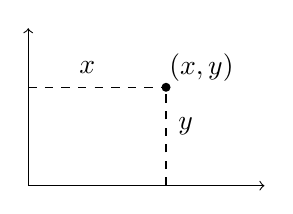
\begin{tikzpicture}
			\draw[->] (0,0) -- (3,0);
			\draw[->] (0,0) -- (0,2);
			
			\draw[dashed] (1.75,0) -- (1.75,1.25);
			\draw[dashed] (0,1.25) -- (1.75,1.25);
			
			\node[draw,circle,inner sep=1pt,fill] at (1.75,1.25) {};
			
			\node at (0.75,1.5) {$x$};
			\node at (2,0.75) {$y$};
			\node at (2.2,1.5) {$(x,y)$};
		\end{tikzpicture}
	\end{center}

	\noindent This is not, however, the only way to define a point in two dimensional space. Instead of moving vertically and horizontally from the origin to get to the point we could instead go straight out of the origin until we hit the point and then determine the angle this line makes with the positive $ x $-axis. We could then use the distance of the point from the origin and the amount we needed to rotate from the positive $ x $-axis as the coordinates of the point. This is shown in the sketch below.
	
	\begin{center}
		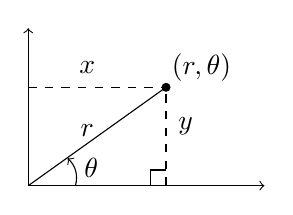
\begin{tikzpicture}
		\draw[->] (0,0) -- (3,0);
		\draw[->] (0,0) -- (0,2);
		
		\draw[dashed] (1.75,0) -- (1.75,1.25);
		\draw[dashed] (0,1.25) -- (1.75,1.25);
		
		\node[draw,circle,inner sep=1pt,fill] at (1.75,1.25) {};
		
		\node at (0.75,1.5) {$x$};
		\node at (2,0.75) {$y$};
		\node at (2.2,1.5) {$(r,\theta)$};
		\node at (0.75,0.7) {$r$};
		\node at (0.8,0.225) {$\theta$};
		
		\draw (0,0) -- (1.75,1.25);
		
		\draw[<-] (0.5,0.35) to[bend left] (0.6,0);
		
		\draw (1.55,0) -- (1.55,0.2);
		\draw (1.55,0.2) -- (1.75,0.2);
		\end{tikzpicture}
	\end{center}
	Coordinates in this form are called \textit{polar coordinates}. Note that $ r $ can be both positive and negative. In polar coordinates the origin is often called the \textit{pole}. Because we aren't actually moving away from the origin/pole we know that $ r = 0 $. However, we can still rotate around the system by any angle we want and so the coordinates of the origin/pole are $ (0,\theta) $.\\ \\
	Now that we've got a grasp on polar coordinates we need to think about converting between the two coordinate systems. Well start out with the following sketch reminding us how both coordinate systems work.
	\begin{center}
		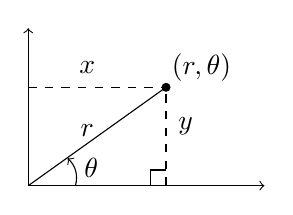
\begin{tikzpicture}
		\draw[->] (0,0) -- (3,0);
		\draw[->] (0,0) -- (0,2);
		
		\draw[dashed] (1.75,0) -- (1.75,1.25);
		\draw[dashed] (0,1.25) -- (1.75,1.25);
		
		\node[draw,circle,inner sep=1pt,fill] at (1.75,1.25) {};
		
		\node at (0.75,1.5) {$x$};
		\node at (2,0.75) {$y$};
		\node at (2.2,1.5) {$(r,\theta)$};
		\node at (0.75,0.7) {$r$};
		\node at (0.8,0.225) {$\theta$};
		
		\draw (0,0) -- (1.75,1.25);
		
		\draw[<-] (0.5,0.35) to[bend left] (0.6,0);
		
		\draw (1.55,0) -- (1.55,0.2);
		\draw (1.55,0.2) -- (1.75,0.2);
		\end{tikzpicture}
	\end{center}
	Note that we've got a right triangle above and with that we can get the following equations that will convert  polar coordinates into Cartesian coordinates.
	\[ x = r\cos\theta \qquad y = r\sin\theta \]
	Converting from Cartesian is almost as easy.  Let's first notice the following.
	\begin{align*}
		x^2 + y^2 &= (r\cos\theta)^2 + (r\sin\theta)^2\\
		&= r^2\cos^2\theta + r^2\sin^2\theta\\
		&= r^2(\cos^2\theta + \sin^2\theta) = r^2
	\end{align*}
	This is a very useful formula that we should remember, however we are after an equation for $ r $ so let's take the square root of both sides. This gives,
	\[ r = \sqrt{x^2 + y^2} \]
	Note that technically we should have a plus or minus in front of the root since we know that $ r $ can be either positive or negative.  We will run with the convention of positive $ r $ here. Getting an equation for $ \theta $ is almost as simple. We'll start with,
	\[ \frac{y}{x} = \frac{r\sin\theta}{r\cos\theta} = \tan\theta \]
	Taking the inverse tangent of both sides gives,
	\[ \theta = \tan^{-1} \left( \frac{y}{x} \right) \]
	Summarizing then gives the following formulas for converting from Cartesian coordinates to polar coordinates.
	\[ r^2 = x^2 + y^2 \]
	\[ \theta = \tan^{-1} \left( \frac{y}{x} \right) \]
	
	
	\section{Tangents with Polar Coordinates}
	
	Now that we have a grasp on polar coordinates we now need to discuss some calculus topics in terms of polar coordinates. \\ \\
	We will start with finding tangent lines to polar curves. In this case we are going to assume that the equation is in the form $ r = f(\theta) $. With the equation in this form we can actually use the equation for the derivative $ \dfrac{dy}{dx} $ we derived when we looked at tangent lines with parametric equations. To do this however requires us to come up with a set of parametric equations to represent the curve. This is actually pretty easy to do.\\ \\
	From our work in the previous section we have the following set of conversion equations for going from polar coordinates to Cartesian coordinates.
	\[ x = r\cos\theta \qquad y = r\sin\theta \]
	Now, we'll use the fact that we're assuming that the equation is in the form $ r = f(\theta) $. Substituting this into these equations gives the following set of parametric equations (with $ \theta $ as the parameter) for the curve.
	\[ x = f(\theta)\,\cos\theta \qquad y = f(\theta)\,\sin\theta \]
	Now, we will need the following derivatives.
	\begin{align*}
		\frac{dx}{d\theta} & = f'(\theta)\,\cos\theta - f(\theta)\,\sin\theta & \frac{dy}{d\theta} & = f'(\theta)\,\sin\theta - f(\theta)\,\cos\theta \\
		                   & = \frac{dr}{d\theta} \cos\theta - r\sin\theta    &                    & = \frac{dr}{d\theta} \sin\theta - r\cos\theta
	\end{align*}
	The derivative $ \dfrac{dy}{dx} $ is then
	\[ \frac{dy}{dx} = \frac{\dfrac{dy}{d\theta}}{\dfrac{dx}{d\theta}} = \frac{\dfrac{dr}{d\theta} \sin\theta - r\cos\theta}{\dfrac{dr}{d\theta} \cos\theta - r\sin\theta} \]
	
	
	\section{Area with Polar Coordinates}
	
	In this section we are going to look at areas enclosed by polar curves. Note as well that we said ``enclosed by'' instead of ``under'' as we typically have in these problems. These problems work a little differently in polar coordinates. Here is a sketch of what the area that we'll be finding in this section looks like.
	\begin{center}
		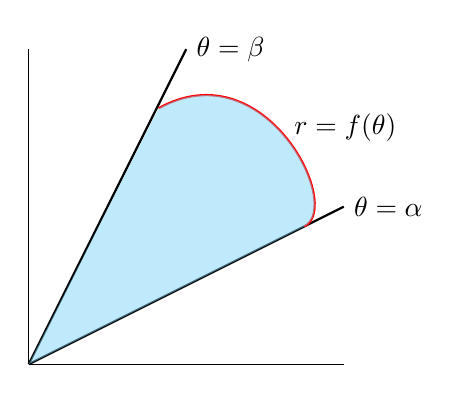
\begin{tikzpicture}
		\draw (0,0) -- (4,0);
		\draw (0,0) -- (0,4);
		
		% Angle parameters
		\draw[thick] (0,0) -- (2,4) node[right] {$\theta = \beta$};
		\draw[thick] (0,0) -- (4,2) node[right] {$\theta = \alpha$};
		
		% Curves
		\draw[thick,draw=red] (1.65,3.25) .. controls(3,4) and (4,2) .. (3.5,1.75);
		
		% Area
		\fill[cyan!50,opacity=0.5] (0,0) -- (1.65,3.25) .. controls(3,4) and (4,2) .. (3.5,1.75);
		
		% Nodes
		\draw (3.25,3) node[right] {$r = f(\theta)$};
		
		\end{tikzpicture}
	\end{center}
	We'll be looking for the shaded area in the sketch above. The formula for finding this area is,
	\[ A = \int_{\alpha}^{\beta} \frac{1}{2}r^2\,d\theta \]
	So, that's how we determine areas that are enclosed by a single curve, but what about situations like the following sketch were we want to find the area between two curves.
		\begin{center}
		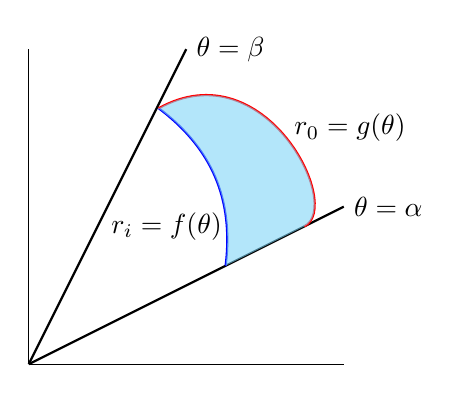
\begin{tikzpicture}
		\draw (0,0) -- (4,0);
		\draw (0,0) -- (0,4);
		
		% Angle parameters
		\draw[thick] (0,0) -- (2,4) node[right] {$\theta = \beta$};
		\draw[thick] (0,0) -- (4,2) node[right] {$\theta = \alpha$};
		
		% Curves
		\draw[thick,draw=blue] (1.65,3.25) to[bend left] (2.5,1.25);
		\draw[thick,draw=red] (1.65,3.25) .. controls(3,4) and (4,2) .. (3.5,1.75);
		
		% Area
		\fill[cyan!50,opacity=0.6] (1.65,3.25) to[bend left] (2.5,1.25) -- (2.5,1.25) -- (3.5,1.75) -- (1.65,3.25) .. controls(3,4) and (4,2) .. (3.5,1.75);
		
		% Nodes
		\draw (3.25,3) node[right] {$r_0 = g(\theta)$};
		\draw (1.75,1.75) node {$r_i = f(\theta)$};
		
		\end{tikzpicture}
	\end{center}
	In this case we can use the above formula to find the area enclosed by both and then the actual area is the difference between the two.  The formula for this is,
	\[ A = \int_{\alpha}^{\beta} \frac{1}{2} (r_0^2 - r_i^2)\,d\theta \]
	
	
	\section{Arc Length with Polar Coordinates}
	
	In this section we'll look at the arc length of the curve given by,
	\[ r = f(\theta) \qquad \alpha \leq \theta \leq \beta \]
	where we also assume that the curve is traced out exactly once. Just as we did with the tangent lines in polar coordinates we’ll first write the curve in terms of a set of parametric equations,
	\begin{align*}
		x &= r\cos\theta   &    y &= r\sin\theta\\
		&= f(\theta)\cos\theta  &   &= f(\theta)\sin\theta
	\end{align*}
	and we can now use the parametric formula for finding the arc length.\\ \\
	We'll need the following derivatives for these computations.
	\begin{align*}
		\frac{dx}{d\theta} & = f'(\theta)\,\cos\theta - f(\theta)\,\sin\theta & \frac{dy}{d\theta} & = f'(\theta)\,\sin\theta - f(\theta)\,\cos\theta \\
		& = \frac{dr}{d\theta} \cos\theta - r\sin\theta    &                    & = \frac{dr}{d\theta} \sin\theta - r\cos\theta
	\end{align*}
	We'll need the following for our $ ds $.
	\begin{align*}
		\left(\frac{dx}{d\theta} \right)^2 + \left( \frac{dy}{d\theta} \right)^2 &= \left( \frac{dr}{d\theta} \cos\theta - r\sin\theta \right)^2 + \left( \frac{dr}{d\theta} \sin\theta - r\cos\theta \right)^2\\
		&= \left(\frac{dr}{d\theta}\right)^2 \cos^2\theta - 2r\frac{dr}{d\theta}\cos\theta \sin\theta + r^2\sin^2\theta \\
		& \qquad \qquad  \qquad + \left(\frac{dr}{d\theta} \right)^2 \sin^2\theta + 2r\frac{dr}{d\theta} \cos\theta \sin\theta + r^2\cos^2\theta \\
		&= \left( \frac{dr}{d\theta}\right)^2 (\cos^2\theta + \sin^2\theta) + r^2(\cos^2\theta + \sin^2\theta) \\
		&= r^2 + \left( \frac{dr}{d\theta}\right)^2
	\end{align*}
	The arc length formula for polar coordinates is then,
	\[ L = \int ds \]
	where
	\[ ds = \sqrt{r^2 + \left( \frac{dr}{d\theta}\right)^2} \, d\theta \]
	
	
	\section{Surface Area with Polar Coordinates}
	
	We will be looking at surface area in polar coordinates in this section. Note however that all we're going to do is give the formulas for the surface area since most of these integrals tend to be fairly difficult.\\ \\
	We want to find the surface area of the region found by rotating,
	\[ r = f(\theta) \qquad \alpha \leq \theta \leq \beta  \]
	about the $ x $ or $ y $-axis.\\ \\
	As we did in the tangent and arc length sections we'll write the curve in terms of a set of parametric equations.
	\begin{align*}
		x &= r\cos\theta  &  y &= r\sin\theta\\
		&= f(\theta)\cos\theta  &  &= f(\theta) \sin\theta
	\end{align*}
	If we now use the parametric formula for finding the surface area we'll get,
	\[ S = \int 2\pi y\,ds \qquad \text{rotation about } x \text{-axis} \]
	\[ S = \int 2\pi x\,ds \qquad \text{rotation about } y \text{-axis} \]
	where,
	\[ ds = \sqrt{r^2 + \left( \frac{dr}{d\theta}\right)^2} \, d\theta \qquad r=f(\theta), \, \alpha \leq \theta \leq \beta \]
	Note that because we will pick up a $ d\theta $ from the $ ds $ we'll need to substitute one of the parametric equations in for $ x $ or $ y $ depending on the axis of rotation. This will often mean that the integrals will be somewhat unpleasant.
	
	
	
	\chapter{Sequences and Series}
	
	\section{Sequences}
	
	Let's start off this section with a discussion of just what a sequence is. A sequence is nothing more than a list of numbers written in a specific order. The list may or may not have an infinite number of terms in them although we will be dealing exclusively with infinite sequences in this class. General sequence terms are denoted as follows,
	\begin{align*}
		& a_1 - \text{first term}\\
		& a_2 - \text{second term}\\
		& \qquad \qquad \vdots \\
		& a_n - n^{th} \text{ term}\\
		& a_{n+1} - (n+1)^{th} \text{ term}\\
		& \qquad \qquad \vdots 
	\end{align*}
	Because we will be dealing with infinite sequences each term in the sequence will be followed by another term as noted above. In the notation above we need to be very careful with the subscripts. The subscript of $ n+1 $ denotes the next term in the sequence and NOT one plus the $ n^{th} $ term!  In other words,
	\[ a_{n+1} \neq a_n + 1 \]
	so be very careful when writing subscripts to make sure that the ``+1'' doesn't migrate out of the subscript! This is an easy mistake to make when you first start dealing with this kind of thing.\\ \\
	There is a variety of ways of denoting a sequence. Each of the following are equivalent ways of denoting a sequence.
	\[ \{ a_1,a_2,a_3,\ldots , a_n,a_{n+1},\ldots  \} \qquad \{ a_n \} \qquad \{ a_n \}_{n=1}^{\infty} \]
	In the second and third notations above $ a_n $ is usually given by a formula. \\ \\
	One very important thing to note about sequences is to treat the sequence terms as functions and plotting them will allow us to do many things with sequences that we couldn't do otherwise. Before delving further into this idea however we need to get a couple more ideas out of the way.\\ \\
	First we want to think about ``graphing'' a sequence. To graph the sequence $ \{ a_n \} $ we plot the points $ (n,a_n) $ as $ n $ ranges over all possible values on a graph. For instance, let's graph the sequence $ \left\{ \dfrac{n+1}{n^2} \right\}_{n=1}^{\infty} $. The first few points on the graph are,
	\[ (1,2), \left(2,\frac{3}{4} \right), \left(3,\frac{4}{9}\right), \left(4,\frac{5}{16}\right), \left(5, \frac{6}{25}\right), \ldots \]
	The graph, for the first 30 terms of the sequence, is then,
	
	\begin{center}
		\begin{tikzpicture}[scale=0.75]
		\begin{axis}[
		axis lines=middle,
		xlabel={$n$},
		x label style={at={(axis description cs:0.5,-0.1)},anchor=north},
		scatter/classes={%
			a={draw=red,fill=red}}]
		\addplot[scatter,only marks,%
		scatter src=explicit symbolic]%
		table[meta=label] {
			x y label
			1 2 a
			2 0.75 a
			3 0.44 a
			4 0.3125 a
			5 0.24 a
			6 0.194 a
			7 0.163 a
			8 0.1406 a
			9 0.1234 a
			10 0.11 a
			11 0.099 a
			12 0.090 a
			13 0.08284 a
			14 0.0765 a
			15 0.0711 a
			16 0.0664 a 
			17 0.0622 a
			18 0.0586 a
			19 0.0554 a
			20 0.0525 a
			21 0.0498 a
			22 0.0475 a
			23 0.04536 a
			24 0.0434 a
			25 0.0416 a
			26 0.0399 a
			27 0.0384 a
			28 0.03699 a
			29 0.03567 a
			30 0.03444 a
		};
		\end{axis}
		\end{tikzpicture}
	\end{center}
	This graph leads us to an important idea about sequences.  Notice that as $ n $ increases the sequence terms in our sequence, in this case, get closer and closer to zero. We then say that zero is the limit (or sometimes the limiting value) of the sequence and write,
	\[ \lim\limits_{n\to \infty} a_n = \lim\limits_{n\to \infty} \frac{n+1}{n^2} = 0 \]
	This notation should look familiar to you. It is the same notation we used when we talked about the limit of a function. In fact, if you recall, we said earlier that we could think of sequences as functions in some way and so this notation shouldn't be too surprising.\\ \\
	Using the ideas that we developed for limits of functions we can write down the following \textit{working} definition for limits of sequences.\\ \\
	\textbf{\textit{Working} Definition of Limit}
	\begin{enumerate}
		\item We say that $ \lim\limits_{n \to \infty} a_n = L $ if we can make $ a_n $ as close to $ L $ as we want for all sufficiently large $ n $. In other words, the value of the $ a_n $'s approach $ L $ as $ n $ approaches infinity.
		
		\item We say that $ \lim\limits_{n \to \infty} a_n = \infty $ if we can make $ a_n $ as large as we want for all sufficiently large $ n $. Again, in other words, the value of the $ a_n $'s get larger and larger without bound as $ n $ approaches infinity.
		
		\item We say that $ \lim\limits_{n \to \infty} a_n = -\infty $ if we can make $ a_n $ as large and negative as we want for all sufficiently large $ n $. Again, in other words, the value of the $ a_n $'s are negative and get larger and larger without bound as $ n $ approaches infinity.
	\end{enumerate}
	The working definitions of the various sequence limits are nice in that they help us to visualize what the limit actually is. Just like with limits of functions however, there is also a precise definition for each of these limits. Let's give those before proceeding\\ \\
	\textbf{\textit{Precise} Definition of Limit}
	\begin{enumerate}
		\item We say that $ \lim\limits_{n \to \infty} a_n = L $ if for every number $ \varepsilon > 0 $ there is an integer $ N $ such that $ |a_n - L| < \varepsilon $ whenever $ n > N $.
		
		\item We say that $ \lim\limits_{n \to \infty} a_n = \infty  $ if for every number $ M > 0 $ there is an integer $ N $ such that $ a_n > M $ whenever $ n > N $.
		
		\item We say that $ \lim\limits_{n \to \infty} a_n = -\infty $ if for every number $ M < 0 $ there is an integer $ N $ such that $ a_n < M $ whenever $ n > N $.
	\end{enumerate}
	We won't be using the precise definition often, but it will show up occasionally. Note that both definitions tell us that in order for a limit to exist and have a finite value all the sequence terms must be getting closer and closer to that finite value as $ n $ increases.\\ \\
	Now that we have the definitions of the limit of sequences out of the way we have a bit of terminology that we need to look at. If $ \lim\limits_{n \to \infty} a_n  $ exists and is finite we say that the sequence is \textit{convergent}. If $ \lim\limits_{n \to \infty} a_n  $ doesn't exist or is infinite we say the sequence \textit{diverges}. Note that sometimes we will say the sequence \textit{diverges to} $ \infty $ if $ \lim\limits_{n \to \infty} a_n = \infty $ and if $ \lim\limits_{n \to \infty} a_n = -\infty $ we will sometimes say that the sequence \textit{diverges to} $ -\infty $.\\ \\
	So just how do we find the limits of sequences? Most limits of most sequences can be found using one of the following theorems.
	\begin{theorem}
		Given the sequence $ \{ a_n \} $ if we have a function $ f(x) $ such that $ f(n) = a_n $ and $ \lim\limits_{n \to \infty} f(n) = L $ then $ \lim\limits_{n \to \infty} a_n = L $.
	\end{theorem}
	\noindent This theorem is basically telling us that we take the limits of sequences much like we take the limit of functions. In fact, in most cases we'll not even really use this theorem by explicitly writing down a function. We will more often just treat the limit as if it were a limit of a function and take the limit as we always did back in Calculus I when we were taking the limits of functions.\\ \\
	So, now that we know that taking the limit of a sequence is nearly identical to taking the limit of a function we also know that all the properties from the limits of functions will also hold.\\ \\
	\textbf{Properties}
	
	\begin{enumerate}
		\item $ \lim\limits_{n \to \infty} (a_n \pm b_n) = \lim\limits_{n \to \infty} a_n \pm \lim\limits_{n \to \infty} b_n $
		
		\item $  \lim\limits_{n \to \infty} c a_n = c \lim\limits_{n \to \infty} a_n $, where $ c \in \R $.
		
		\item $ \lim\limits_{n \to \infty} (a_n b_n) = \left( \lim\limits_{n \to \infty} a_n \right) \left( \lim\limits_{n \to \infty} b_n\right) $
		
		\item $ \lim\limits_{n \to \infty} \dfrac{a_n}{b_n} = \dfrac{\lim\limits_{n \to \infty} a_n}{\lim\limits_{n \to \infty} b_n} $, provided $ \lim\limits_{n \to \infty} b_n \neq 0 $.
		
		\item $ \lim\limits_{n \to \infty} (a_n)^p = \left( \lim\limits_{n \to \infty} a_n \right)^p $, provided $ a_n \geq 0 $.
	\end{enumerate}
	These properties can be proved using Theorem 4.1.1 above and the function limit properties we saw in Calculus I or we can prove them directly using the precise definition of a limit using nearly identical proofs of the function limit properties.\\ \\ 
	Next, just as we had a Squeeze Theorem for function limits we also have one for sequences and it is pretty much identical to the function limit version.
	\begin{theorem}[Squeeze Theorem for Sequences]
		If $ a_n  \leq c_n \leq b_n $ for some $ n > N $ and $ \lim\limits_{n \to \infty} a_n = \lim\limits_{n \to \infty} b_n = L $ then $ \lim\limits_{n \to \infty} c_n = L $.
	\end{theorem}

	\noindent As we'll see not all sequences can be written as functions that we can actually take the limit of. This will be especially true for sequences that alternate in signs. While we can always write these sequence terms as a function we simply don’t know how to take the limit of a function like that. The following theorem will help with some of these sequences.
	\begin{theorem}
		If $ \lim\limits_{n \to \infty} |a_n| = 0 $ then $ \lim\limits_{n \to \infty} a_n = 0 $.
	\end{theorem}
	\begin{proof}
		The main thing to this proof is to note that 
		\[ -|a_n| \leq a_n \leq |a_n| \]
		Then note that
		\[ \lim\limits_{n \to \infty} (-|a_n|) = - \lim\limits_{n \to \infty} |a_n| = 0 \]
		We then have $ \lim\limits_{n \to \infty} (-|a_n|) = \lim\limits_{n \to \infty} |a_n| = 0 $ and so by the Squeeze Theorem we must also have that $ \lim\limits_{n \to \infty} a_n = 0 $.
	\end{proof}
	
	\section{More on Sequences}
	
	In the previous section we introduced the concept of a sequence and talked about limits of sequences and the idea of convergence and divergence for a sequence. In this section we want to take a quick look at some ideas involving sequences. Let's start off with some terminology and definitions.
	Given any sequence $ \{ a_n \} $ we have the following:
	\begin{enumerate}
		\item We call the sequence \textit{increasing} if $ a_n < a_{n+1} $ for every $ n $.
		\item We call the sequence \textit{decreasing} if $ a_n > a_{n+1} $ for every $ n $.
		\item If $ \{ a_n \} $ is an increasing sequence or $ \{ a_n \} $ is a decreasing sequence we call it \textit{monotonic}.
		\item If there exists a number $ m $ such that $ m \leq a_n $ for every $ n $ we say the sequence is \textit{bounded below}. The number $ m $ is sometimes called a \textit{lower bound} for the sequence.
		\item If there exists a number $ M $ such that $ a_n \leq M $ for every $ n $ we say the sequence is \textit{bounded above}. The number $ M $ is sometimes called an \textit{upper bound} for the sequence.
		\item If the sequence is both bounded below and bounded above we call the sequence \textit{bounded}.
	\end{enumerate}
	Note that in order for a sequence to be increasing or decreasing it must be increasing/decreasing for every $ n $. In other words, a sequence that increases for three terms and then decreases for the rest of the terms is NOT a decreasing sequence! Also note that a monotonic sequence must always increase or it must always decrease.\\ \\
	We'll close out this section with a nice theorem that we'll use in some of the proofs later in this chapter.
	\begin{theorem}
		If $ \{ a_n \} $ is bounded and monotonic then $ \{ a_n \} $ is convergent.
	\end{theorem}

	\section{Series - The Basics}
	
	In this section we will introduce the topic that we will be discussing for the rest of this chapter. That topic is infinite series. So just what is an infinite series? Well, let's start with a sequence $ \{a_n \}_{n=1}^{\infty} $ (note the  is for convenience, it can be anything) and define the following,
	\begin{align*}
		s_1 &= a_1\\
		s_2 &= a_1 + a_2\\
		s_3 &= a_1 + a_2 + a_3\\
		s_4 &= a_1 + a_2 + a_3 + a_4\\
			& \qquad \qquad \vdots\\
		s_n &= a_1 + a_2 + a_3 + a_4 + \ldots + a_n = \sum\limits_{i=1}^{\infty} a_i
	\end{align*}
	The $ s_n $ are called \textit{partial sums} and notice they form a sequence, $ \{ s_n \}_{n=1}^{\infty} $. Also recall that the $ \Sigma $ is used to represent this summation and called a variety of names. The most common names are: \textit{series notation, summation notation,} and \textit{sigma notation}. We want to take a look at the limit of the sequence of partial sums, $ \{ s_n \}_{n=1}^{\infty} $. Notationally we'll define,
	\[ \lim\limits_{n \to \infty} s_n = \lim\limits_{n \to \infty} \sum\limits_{i=1}^{n} a_i = \sum\limits_{i=1}^{\infty} a_i \]
	We call $ \sum\limits_{i=1}^{\infty} a_i $ an \textit{infinite series} and note that the series starts at $ i = 1 $ because that is where our original sequence, $ \{ a_n \}_{i=1}^{\infty} $, started. If the sequence of partial sums, $ \{ s_n \}_{n=1}^{\infty} $, is convergent and its limit is finite then we also call the infinite series, $ \sum\limits_{i=1}^{\infty} a_i $ \textit{convergent} and if the sequence of partial sums is divergent then the infinite series is also called \textit{divergent}. In the next section we're going to be discussing in greater detail the value of an infinite series, provided it has one of course as well as the ideas of convergence and divergence. This section is going to be devoted mostly to notational issues as well as making sure we can do some basic manipulations with infinite series so we are ready for them when we need to be able to deal with them in later sections.\\ \\
	Now, in $ \sum\limits_{i=1}^{\infty} a_i $ the $ i $ is called the \textit{index of summation} or just index for short and note that the letter we use to represent the index does not matter. So for example the following series are all the same. The only difference is the letter we've used for the index.
	\[ \sum\limits_{i=0}^{\infty} \frac{2^i}{i^2 + 1} = \sum\limits_{k=0}^{\infty} (-1)^k \frac{k!}{k+1} = \sum\limits_{n=0}^{\infty} \frac{3}{n^2 + 5} \, \, etc   \]
	It is important to again note that the index will start at whatever value the sequence of series terms starts at and this can literally be anything. So far we've used $ n=0 $ and $ n=1 $ but the index could have started anywhere. In fact, we will usually use $ \sum a_n $ to represent an infinite series in which the starting point for the index is not important. When we drop the initial value of the index we'll also drop the infinity from the top so don't forget that it is still technically there.\\ \\
	We will be dropping the initial value of the index in quite a few facts and theorems that we'll be seeing throughout this chapter. In these facts/theorems the starting point of the series will not affect the result and so to simplify the notation and to avoid giving the impression that the starting point is important we will drop the index from the notation. Do not forget however, that there is a starting point and that this will be an infinite series.\\ \\
	Now that some of the notational issues are out of the way we need to start thinking about various ways that we can manipulate series. We'll start this off with basic arithmetic with infinite series as we’ll need to be able to do that on occasion. We have the following properties.\\ \\
	\textbf{Properties}\\
	If $ \sum a_n $ and $ \sum b_n $ are both convergent series then,
	\begin{enumerate}
		\item $ \sum c a_n $, where $ c $ is any number, is also convergent and $ \sum c a_n = c \sum a_n $
		
		\item $ \sum\limits_{k=n}^{\infty} a_n \pm \sum\limits_{k=n}^{\infty} b_n $ is also convergent and $ \sum\limits_{k=n}^{\infty} a_n \pm \sum\limits_{k=n}^{\infty} b_n = \sum\limits_{k=n}^{\infty} (a_n \pm b_n) $.
	\end{enumerate}
	Before we move on to a different topic let's discuss multiplication of series briefly. We'll start both series at $ n=0 $ for a later formula and then note that,
	\[ \left( \sum\limits_{n=0}^{\infty} a_n \right)  \left( \sum\limits_{n=0}^{\infty} b_n \right) \neq \sum\limits_{n=0}^{\infty} a_n b_n \]
	With multiplication we're really asking us to do the following,
	\[ \left( \sum\limits_{n=0}^{\infty} a_n \right)  \left( \sum\limits_{n=0}^{\infty} b_n \right) = (a_0 + a_1 + a_2 + a_3 + \ldots) (b_0 + b_1 + b_2 + b_3 + \ldots) \]
	The next topic that we need to discuss in this section is that of \textit{index shift}. Despite the fact that we won't use it much in this course doesn't mean however that it isn't used often in other classes where you might run across series. So, we will cover it briefly here so that you can say you've seen it.\\ \\
	The basic idea behind index shifts is to start a series at a different value for whatever the reason (and yes, there are legitimate reasons for doing that). Consider the following series,
	\[ \sum\limits_{n=2}^{\infty} \frac{n+5}{2^n} \]
	Suppose that for some reason we wanted to start this series at $ n=0 $, but we didn't want to change the value of the series. This means that we can't just change the $ n=2 $ to $ n=0 $, as this would add in two new terms to the series and thus change its value.\\ \\
	Performing an index shift is a fairly simple process to do. We'll start by defining a new index, say $ i $, as follows,
	\[ i = n-2 \]
	Now, when $ n=2 $, we will get $ i=0 $. Notice as well that if $ n=\infty $ then $ i = \infty - 2 = \infty $, so only the lower limit will change here. Next, we can solve this for $ n $ to get,
	\[ n = i + 2 \]
	We can now completely rewrite the series in terms of the index $ i $ instead of the index $ n $ simply by plugging in our equation for $ n $ in terms of $ i $.
	\[ \sum\limits_{n=2}^{\infty} \frac{n+5}{2^n} = \sum\limits_{i=0}^{\infty} \frac{(i+2)+5}{2^{i+2}} = \sum\limits_{i=0}^{\infty} \frac{i+7}{2^{i+2}} \]
	To finish the problem out we'll recall that the letter we used for the index doesn't matter and so we'll change the final $ i $ back into an $ n $ to get,
	\[ \sum\limits_{n=0}^{\infty} \frac{n+7}{2^{n+2}} \]
	The final topic in this section is again a topic that we'll not be seeing all that often in this class, although we will be seeing it more often than the index shifts. This final topic is really more about alternate ways to write series when the situation requires it.\\ \\
	Let's start with the following series and note that the $ n=1 $ starting point is only for convenience since we need to start the series somewhere. 
	\[ \sum\limits_{n=1}^{\infty} a_n = a_1 + a_2 + a_3 + a_4 + \ldots \]
	Notice that if we ignore the first term the remaining terms will also be a series that will start at $ n=2 $ instead of $ n=1 $. So, we can rewrite the original series as follows,
	\[ \sum\limits_{n=1}^{\infty} a_n = a_1 + \sum\limits_{n=2}^{\infty} a_n  \]
	In this example we say that we’ve stripped out the first term. We could have stripped out more terms if we wanted to. In the following series we've stripped out the first two terms and the first four terms respectively.
	\begin{align*}
		\sum\limits_{n=1}^{\infty} a_n &= a_1 + a_2 + \sum\limits_{n=3}^{\infty} a_n\\
		\sum\limits_{n=1}^{\infty} a_n &= a_1 + a_2 + a_3 + a_4 + \sum\limits_{n=5}^{\infty} a_n
	\end{align*}
	Being able to strip out terms will, on occasion, simplify our work or allow us to reuse a prior result so it's an important idea to remember.

	\section{Series - Convergence/Divergence}
	
	In the previous section we spent some time getting familiar with series and we briefly defined convergence and divergence. Before worrying about convergence and divergence of a series we wanted to make sure that we've started to get comfortable with the notation involved in series and some of the various manipulations of series that we will, on occasion, need to be able to do.\\ \\
	So, let's recap just what an infinite series is and what it means for a series to be convergent or divergent. We'll start with a sequence $ \{ a_n \}_{n=1}^{\infty} $ and again note that we're starting the sequence at $ n=1 $ only for the sake of convenience and it can, in fact, be anything. Next we define the partial sums of the series as,
	\begin{align*}
	s_1 &= a_1\\
	s_2 &= a_1 + a_2\\
	s_3 &= a_1 + a_2 + a_3\\
	s_4 &= a_1 + a_2 + a_3 + a_4\\
	& \qquad \qquad \vdots\\
	s_n &= a_1 + a_2 + a_3 + a_4 + \ldots + a_n = \sum\limits_{i=1}^{\infty} a_i
	\end{align*}
	and these form a new sequence, $ \{ s_n \}_{n=1}^{\infty} $.\\ \\
	An infinite series, or just series here since almost every series that we'll be looking at will be an infinite series, is then the limit of the partial sums. Or,
	\[ \sum\limits_{i=1}^{n} a_i = \lim\limits_{n\ to \infty} s_n \]
	If the sequence of partial sums is a convergent sequence (i.e. its limit exists and is finite) then the series is also called \textit{convergent} and in this case if $ \lim\limits_{n \to \infty} s_n = s $ then, $ \sum_{i = 1}^{n} a_i = s $.  Likewise, if the sequence of partial sums is a divergent sequence (i.e. its limit doesn’t exist or is plus or minus infinity) then the series is also called \textit{divergent}.\\ \\
	Here are some examples:
	\begin{center}
		\begin{tabular}{ll}
			$ \lim\limits_{n \to \infty} n = \infty $ & this series diverges\\[3ex]
			$ \lim\limits_{n \to \infty} \dfrac{1}{n^2 - 1} = 0 $ & this series converges\\[3ex]
			$ \lim\limits_{n \to \infty} (-1)^n $ does not exist & this series diverges\\[3ex]
			$ \lim\limits_{n \to \infty} \dfrac{1}{3^{n-1}} = 0 $ & this series converges
		\end{tabular}		
	\end{center}
	Notice that for the two series that converged the series term itself was zero in the limit. This will always be true for convergent series and leads to the following theorem.
	\begin{theorem}
		If $ \sum a_n $ converges then $ \lim\limits_{n\ to \infty} a_n = 0 $.
	\end{theorem}
	\begin{proof}
		First let's suppose that the series starts at $ n=1 $. Then the partial sums are,
		\[ s_{n-1} = \sum\limits_{i=1}^{n-1} a_i = a_1 + a_2 + a_3 + \ldots + a_{n-1} \qquad s_{n} = \sum\limits_{i=1}^{n} a_i = a_1 + a_2 + a_3 + \ldots + a_{n-1} + a_n \]
		Next, we can use these two partial sums to write,
		\[ a_n = s_n - s_{n-1} \]
		Now because we know that $ \sum a_n $ is convergent we also know that the sequence $ \{ s_n \}_{n=1}^{\infty} $ is also convergent and that $ \lim\limits_{n \to \infty} s_n =s $ for some finite value $ s $. However, since $ n-1 \to \infty $ as $ n \to \infty $ we also have $ \lim\limits_{n \to \infty} s_{n-1} = s $. We now have,
		\[ \lim\limits_{n \to \infty} a_n = \lim\limits_{n \to \infty} (s_n - s_{n-1}) = \lim\limits_{n \to \infty} s_n - \lim\limits_{n \to \infty} s_{n-1} = s-s = 0 \]
	\end{proof}
	\noindent Be careful to not misuse this theorem! This theorem gives us a requirement for convergence but not a guarantee of convergence.  In other words, the converse is NOT true. If $ \lim\limits_{n \to \infty} a_n = 0 $ the series may actually diverge! Consider the following two series.
	\[ \sum\limits_{n=1}^{\infty} \frac{1}{n} \qquad \qquad \sum\limits_{n=1}^{\infty} \frac{1}{n^2} \]
	In both cases the series terms are zero in the limit as $ n $ goes to infinity, yet only the second series converges. The first series diverges. It will be a couple of sections before we can prove this, so at this point please believe this and know that you'll be able to prove the convergence of these two series in a couple of sections.\\ \\
	Again, as noted above, all this theorem does is give us a requirement for a series to converge. In order for a series to converge the series terms must go to zero in the limit. If the series terms do not go to zero in the limit then there is no way the series can converge since this would violate the theorem.\\ \\
	This leads us to the first of many tests for the convergence/divergence of a series that we'll be seeing in this chapter.\\ \\
	\textbf{Divergence Test}\\
	If $ \lim\limits_{n \to \infty} a_n \neq 0 $ then $ \sum a_n $ will diverge.\\ \\ \\
	Again, do NOT misuse this test. This test only says that a series is guaranteed to diverge if the series terms don’t go to zero in the limit. If the series terms do happen to go to zero the series may or may not converge!\\ \\
	The divergence test is the first test of many tests that we will be looking at over the course of the next several sections. You will need to keep track of all these tests, the conditions under which they can be used and their conclusions all in one place so you can quickly refer back to them as you need to.\\ \\
	Now, since the main topic of this section is the convergence of a series we should mention a stronger type of convergence. A series $ \sum a_n $ is said to \textit{converge absolutely} if $ \sum |a_n| $ also converges. Absolute convergence is stronger than convergence in the sense that a series that is absolutely convergent will also be convergent, but a series that is convergent may or may not be absolutely convergent. In fact if $ \sum a_n $ converges and $ \sum |a_n| $ diverges the series $ \sum a_n $ is called \textit{conditionally convergent}.
	
	\section{Series - Special Series}
	
	
	In this section we are going to take a brief look at three special series.  Actually, special may not be the correct term. All three have been named which makes them special in some way, however the main reason that we're going to look at two of them in this section is that they are the only types of series that we'll be looking at for which we will be able to get actual values for the series. The third type is divergent and so won't have a value to worry about.\\ \\
	In general, determining the value of a series is very difficult and outside of these two kinds of series that we'll look at in this section we will not be determining the value of series in this chapter.
	
	\subsection*{Geometric Series}
	
	A geometric series is any series that can be written in the form
	\[ \sum\limits_{n=1}^{\infty} ar^{n-1} \qquad \text{or} \qquad \sum\limits_{n=0}^{\infty} ar^n  \]
	If we start with the first form it can be shown that the partial sums are,
	\[ s_n = \frac{a(1 - r^n)}{1-r} = \frac{a}{1-r} - \frac{ar^n}{1-r} \]
	The series will converge provided the partial sums form a convergent sequence, so let's take the limit of the partial sums.
	\begin{align*}
		\lim\limits_{n \to \infty} s_n &= \lim\limits_{n \to \infty}\left( \frac{a}{1-r} - \frac{ar^n}{1-r} \right)\\
		&= \lim\limits_{n \to \infty} \frac{a}{1-r} - \lim\limits_{n \to \infty} \frac{ar^n}{1-r}\\
		&= \frac{a}{1-r} - \frac{a}{1-r} \lim\limits_{n \to \infty} r^n
	\end{align*}
	Now, we know that the limit above will exist and be finite provided $ -1 \leq r \leq 1 $. However, note that we can't let $ $ r=1 $ $ since this will give division by zero. Therefore, this will exist and be finite provided $ -1 < r < 1 $ and in this case the limit is zero and so we get,
	\[ \lim\limits_{n \to \infty} s_n = \lim\limits_{n \to \infty} \frac{a}{1-r} \]
	Therefore, a geometric series will converge if $ -1 < r < 1 $, which is usually written $ |r| < 1 $, its value is,
	\[ \sum\limits_{n=1}^{\infty} ar^{n-1} = \sum\limits_{n=1}^{\infty} ar^n = \frac{a}{1-r} \]
	
	\subsection*{Telescoping Series}
	
	In this portion we are going to look at a series that is called a \textit{telescoping series}. The name in this case comes from what happens with the partial sums and is best shown in an example.\\ \\
	\textbf{Example}: Determine if this series converges or diverges. If it converges find its value
	\[ \sum\limits_{n=0}^{\infty} \frac{1}{n^2 + 3n + 2} \]
	\textit{Solution}. We first need the partial sums for this series.
	\[ s_n = \sum\limits_{i=0}^{n} \frac{1}{i^2 + 3i + 2} \]
	Now, notice that we can use partial fractions on the series term to get,
	\[ \frac{1}{i^2 + 3i + 2} = \frac{1}{(i+2)(i+1)} = \frac{1}{i+1} - \frac{1}{i+2} \]
	So, what does this do for us? Well, let's start writing out the terms of the general partial sum for this series using the partial fraction form.
	\begin{align*}
		s_n &= \sum\limits_{i=0}^{n} \left( \frac{1}{i+1} - \frac{1}{i+2} \right)\\
		&= \left( \frac{1}{1} - \frac{1}{2} \right) + \left( \frac{1}{2} - \frac{1}{3} \right) + \left( \frac{1}{3} - \frac{1}{4} \right) + \cdots + \left( \frac{1}{n} - \frac{1}{n+1} \right) + \left( \frac{1}{n+1} - \frac{1}{n+2} \right)\\
		&= 1 - \frac{1}{n+2}
	\end{align*}
	Notice that every term except the first and last term canceled out. This is the origin of the name \textit{telescoping series}. This also means that we can determine the convergence of this series by taking the limit of the partial sums.
	\[ \lim\limits_{n \to \infty} s_n = \lim\limits_{n \to \infty} \left( 1 - \frac{1}{n+2} \right) = 1 \]
	The sequence of partial sums is convergent and so therefore the series is convergent and has a value of
	\[ \sum\limits_{n=0}^{\infty} \frac{1}{n^2 + 3n + 2} = 1 \]
	Note that it's not always obvious if a series is telescoping or not until you try to get the partial sums and then see if they are in fact telescoping. There is no test that will tell us that we've got a telescoping series right off the bat.  Also note that just because you can do partial fractions on a series term does not mean that the series will be a telescoping series.
	
	\subsection*{Harmonic Series}
	
	This is the third and final series that we’re going to look at in this section.  Here is the \textit{harmonic series}.
	\[ \sum\limits_{n=1}^{\infty} \frac{1}{n} \]
	The harmonic series is divergent and we'll need to wait until the next section to show that. We're also going to use the harmonic series to illustrate a couple of ideas about divergent series that we've already discussed for convergent series. 
	
	\section{Integral Test}
	
	The last topic that we discussed in the previous section was the harmonic series.  In that discussion we stated that the harmonic series was a divergent series. It is now time to prove that statement. This proof will also get us started on the way to our next test for convergence that we'll be looking at.
	So, we will be trying to prove that the harmonic series,
	\[ \sum\limits_{n=1}^{\infty} \frac{1}{n} \]
	diverges. We'll start this off by looking at an apparently unrelated problem.  Let's start off by asking what the area under $ f(x) = \dfrac{1}{x} $ on the interval $ [1,\infty] $. From the section on Improper Integrals we know that this is,
	\[ \int_{1}^{\infty} \frac{1}{x}\,dx = \infty \]
	and so we called this integral divergent (yes, that's the same term we're using here with series...).\\ \\
	So, just how does that help us to prove that the harmonic series diverges? Well, recall that we can always estimate the area by breaking up the interval into segments and then sketching in rectangles and using the sum of the area all of the rectangles as an estimate of the actual area. Let's do that for this problem as well and see what we get.\\ \\
	We will break up the interval into subintervals of width 1 and we'll take the function value at the left endpoint as the height of the rectangle. So, the area under the curve is approximately,
	\begin{align*}
		A &\approx \left( \frac{1}{1} \right) (1) + \left( \frac{1}{2} \right) (1) + \left( \frac{1}{3} \right) (1) + \left( \frac{1}{4} \right) (1) + \left( \frac{1}{5} \right) (1) + \cdots\\
		&= \frac{1}{1} + \frac{1}{2} + \frac{1}{3} + \frac{1}{4} + \frac{1}{5} \cdots\\
		&= \sum\limits_{n=1}^{\infty} \frac{1}{n}
	\end{align*}
	Now note a couple of things about this approximation. First, each of the rectangles overestimates the actual area and secondly the formula for the area is exactly the harmonic series! Putting these two facts together gives the following,
	\[ A \approx \sum\limits_{n=1}^{\infty} \frac{1}{n} > \int_{1}^{\infty} \frac{1}{x} dx = \infty \]
	Since we can't really be larger than infinity the harmonic series must also be infinite in value. In other words, the harmonic series is in fact divergent.\\ \\
	So, we've managed to relate a series to an improper integral that we could compute and it turns out that the improper integral and the series have exactly the same convergence.\\ \\
	Let's see if this will also be true for a series that converges. When discussing the Divergence Test we made the claim that
	\[ \sum\limits_{n=1}^{\infty} \frac{1}{n^2} \]
	converges. Let's see if we can do something similar to the above process to prove this. We will try to relate this to the area under $ f(x) = 1/x^2 $ is on the interval $ [1,\infty] $. Again, from the Improper Integral section we know that,
	\[ \int_{1}^{\infty} \frac{1}{x^2} \, dx = 1 \]
	and so this integral converges. We will once again try to estimate the area under this curve. We will do this in an almost identical manner as the previous part with the exception that instead of using the left end points for the height of our rectangles we will use the right end points. In this case the area estimation is,
	\begin{align*}
		A &\approx \left( \frac{1}{2^2} \right)(1) + \left( \frac{1}{2^2} \right)(1) + \left( \frac{1}{3^2} \right)(1) + \left( \frac{1}{4^2} \right)(1) + \left( \frac{1}{5^2} \right)(1) + \cdots\\
		&= \frac{1}{2^2} + \frac{1}{3^2} + \frac{1}{4^2} + \frac{1}{5^2} + \cdots 
	\end{align*}
	This time, unlike the first case, the area will be an underestimation of the actual area and the estimation is not quite the series that we are working with. Notice however that the only difference is that we're missing the first term.  This means we can do the following,
	\[
	\sum\limits_{n=1}^{\infty} \frac{1}{n^2} = \frac{1}{1^2} + 
	\underbrace{\frac{1}{2^2} + \frac{1}{3^2} + \frac{1}{4^2} + \frac{1}{5^2} + \cdots}_\text{Area Estimation} < 1 + \int_{1}^{\infty} \frac{1}{x^2}\,dx = 1 + 1 = 2
	\]
	Or, putting all this together we see that,
	\[ \sum\limits_{n=1}^{\infty} \frac{1}{n^2} < 2 \]
	With the harmonic series this was all that we needed to say that the series was divergent. With this series however, this isn't quite enough. For instance $ -\infty < 2 $ and if the series did have a value of $ -\infty $ then it would be divergent (when we want convergent). So, let's do a little more work.\\ \\
	First, let's notice that all the series terms are positive (that's important) and that the partial sums are,
	\[ s_n = \sum\limits_{i=1}^{n} \frac{1}{i^2} \]
	Because the terms are all positive we know that the partial sums must be an increasing sequence. In other words,
	\[ s_n = \sum\limits_{i=1}^{n} \frac{1}{i^2} < s_n = \sum\limits_{i=1}^{n+1} \frac{1}{i^2} = s_{n+1} \]
	In $ s_{n+1} $ we are adding a single positive term onto $ s_n $ and so must get larger. Therefore, the partial sums form an increasing (and hence monotonic) sequence. Also note that, since the terms are all positive, we can say,
	\[ s_n = \sum\limits_{i=1}^{n} \frac{1}{i^2} < s_n = \sum\limits_{n=1}^{\infty} \frac{1}{n^2} < 2 \qquad \Rightarrow \qquad s_n < 2 \]
	and so the sequence of partial sums is a bounded sequence.\\ \\
	In the second section on Sequences we gave a theorem that stated that a bounded and monotonic sequence was guaranteed to be convergent. This means that the sequence of partial sums is a convergent sequence. So, who cares right? Well recall that this means that the series must then also be convergent! So, once again we were able to relate a series to an improper integral (that we could compute) and the series and the integral had the same convergence.\\ \\
	We went through a fair amount of work in both of these examples to determine the convergence of the two series.  Luckily for us we don’t need to do all this work every time.  The ideas in these two examples can be summarized in the following test.\\ \\
	\textbf{Integral Test}\\
	Suppose that $ f(x) $ is a continuous, positive, and decreasing function on the interval $ [k,\infty] $ and that $ f(n) = a_n $ then,
	\begin{enumerate}
		\item If $ \int_{k}^{\infty} f(x)\,dx $ is convergent so is $ \sum\limits_{n=k}^{\infty} a_n $.
		
		\item If $ \int_{k}^{\infty} f(x)\,dx $ is divergent so is $ \sum\limits_{n=k}^{\infty} a_n $.
	\end{enumerate}
	There are a couple of things to note about the integral test. First, the lower limit on the improper integral must be the same value that starts the series.  Second, the function does not actually need to be decreasing and positive everywhere in the interval. All that's really required is that eventually the function is decreasing and positive. In other words, it is okay if the function (and hence series terms) increases or is negative for a while, but eventually the function (series terms) must decrease and be positive for all terms. \\ \\
	We can use the Integral Test to get the following fact/test for some series.\\ \\
	\textbf{P-Series Test}\\
	If $ k > 0 $ then $ \sum\limits_{n=k}^{\infty} \frac{1}{n^p} $ converges if $ p > 1 $ and diverges if $ p \leq 1 $.
	
	
	\section{Comparison Test/Limit Comparison Test}
	
	In the previous section we saw how to relate a series to an improper integral to determine the convergence of a series. While the integral test is a nice test, it does force us to do improper integrals which aren't always easy and in some cases may be impossible to determine the convergence of. For instance consider the following series.
	\[ \sum\limits_{n=0}^{\infty} \frac{1}{3^n + n} \]
	In order to use the Integral Test we would have to integrate
	\[ \int_{0}^{\infty} \frac{1}{3^x + x}\,dx \]
	which is pretty much impossible. Nicely enough for us there is another test that we can use on this series that will be much easier to use.\\ \\
	First, let's note that the series terms are positive. As with the Integral Test that will be important in this section. Next let's note that we must have $ x > 0 $ since we are integrating on the interval $ 0 \leq x \leq \infty $. Likewise, regardless of the value of $ x $ we will always have $ 3^x > 0 $. So, if we drop the $ x $ from the denominator the denominator will get smaller and hence the whole fraction will get larger. So,
	\[ \frac{1}{3^n + n} < \frac{1}{3^n} \]
	Now, notice that
	\[ \sum\limits_{n=0}^{\infty} \frac{1}{3^n} \]
	is a geometric series and we know that since $ |r| = \bigg|\dfrac{1}{3}\bigg| < 1 $ the series will converge and its value will be,
	\[ \sum\limits_{n=0}^{\infty} \frac{1}{3^n} = \frac{1}{1 - \frac{1}{3}} = \frac{3}{2} \]
	Now, if we go back to our original series and write down the partial sums we get,
	\[ s_n = \sum\limits_{i=1}^{n} \frac{1}{3^i + i} \]
	Since all the terms are positive adding a new term will only make the number larger and so the sequence of partial sums must be an increasing sequence.
	\[ s_n = \sum\limits_{i=1}^{n} \frac{1}{3^i + i} < \sum\limits_{i=1}^{n+1} \frac{1}{3^i + i} = s_{n+1} \]
	Then since,
	\[ \frac{1}{3^n + n} < \frac{1}{3^n} \]
	and because the terms in these two sequences are positive we can also say that,
	\[ s_n = \sum\limits_{i=1}^{n} \frac{1}{3^i + i} < \sum\limits_{i=1}^{n} \frac{1}{3^i} < \sum\limits_{n=1}^{\infty} \frac{1}{3^n} = \frac{3}{2} \quad \Rightarrow \quad s_n < \frac{3}{2} \]
	Therefore, the sequence of partial sums is also a bounded sequence. Then from the second section on sequences we know that a monotonic and bounded sequence is also convergent. So, the sequence of partial sums of our series is a convergent sequence. This means that the series itself,
	\[ \sum\limits_{n=0}^{\infty} \frac{1}{3^n + n} \]
	is also convergent.\\ \\
	So, what did we do here? We found a series whose terms were always larger than the original series terms and this new series was also convergent. Then since the original series terms were positive (very important) this meant that the original series was also convergent.\\ \\
	To show that a series (with only positive terms) was divergent we could go through a similar argument and find a new divergent series whose terms are always smaller than the original series. In this case the original series would have to take a value larger than the new series. However, since the new series is divergent its value will be infinite. This means that the original series must also be infinite and hence divergent.\\ \\
	We can summarize all this in the following test.\\ \\
	\textbf{Comparison Test}\\
	Suppose that we have two series $ \sum a_n $ and $ \sum b_n $ with $ a_n,b_n \geq 0 $ for all $ n $ and $ a_n \leq b_n $ for all $ n $. Then,
	\begin{enumerate}
		\item If $ \sum b_n $ is convergent then so is $ \sum a_n $.
		\item If $ \sum a_n $ is divergent then so is $ \sum b_n $.
	\end{enumerate}
	In other words, we have two series of positive terms and the terms of one of the series is always larger than the terms of the other series. Then if the larger series is convergent the smaller series must also be convergent. Likewise, if the smaller series is divergent then the larger series must also be divergent. Note as well that in order to apply this test we need both series to start at the same place. \\ \\
	The comparison test is a nice test that allows us to do problems that either we couldn't have done with the integral test or at the best would have been very difficult to do with the integral test. That doesn't mean that it doesn’t have problems of its own. Consider the following series
	\[ \sum\limits_{n=0}^{\infty} \frac{1}{3^n - n} \]
	This is not much different from the first series that we looked at. The original series converged because the $ 3^n $ gets very large very fast and will be significantly larger than the $ n $. Therefore, the $ n $ doesn't really affect the convergence of the series in that case. The fact that we are now subtracting the $ n $ off instead of adding the $ n $ on really shouldn't change the convergence. We can say this because the $ 3^n $ gets very large very fast and the fact that we're subtracting $ n $ off won't really change the size of this term for all sufficiently large values of $ n $.\\ \\
	So, we would expect this series to converge. However, the comparison test won't work with this series. To use the comparison test on this series we would need to find a larger series that we could easily determine the convergence of. In this case we can't do what we did with the original series. If we drop the $ n $ we will make the denominator larger (since the $ n $ was subtracted off) and so the fraction will get smaller and just like when we looked at the comparison test for improper integrals knowing that the smaller of two series converges does not mean that the larger of the two will also converge.\\ \\
	So, we will need something else to do help us determine the convergence of this series. The following variant of the comparison test will allow us to determine the convergence of this series.\\ \\
	\textbf{Limit Comparison Test}\\
	Suppose that we have two series $ \sum a_n $ and $ \sum b_n $ with $ a_n \geq 0 $, $ b_n > 0 $ for all $ n $. Define
	\[ c = \lim\limits_{n \to \infty} \frac{a_n}{b_n} \]
	If $ c $ is positive ($ i.e. $ $ c > 0 $) and is finite ($ i.e. $ $ c < \infty $) then either both series converge or both series diverge.
	
	\section{Alternating Series Test}
	
	The last two tests that we looked at for series convergence have required that all the terms in the series be positive. Of course there are many series out there that have negative terms in them and so we now need to start looking at tests for these kinds of series.\\ \\
	The test that we are going to look into in this section will be a test for alternating series. An alternating series is any series, $ \sum a_n $, for which the series terms can be written in one of the following two forms.
	\begin{align*}
		& a_n = (-1)^n b_n \qquad  \quad b_n \geq 0\\
		& a_n = (-1)^{n+1} b_n \qquad b_n \geq 0
 	\end{align*}
	
	\noindent \textbf{Alternating Series Test}\\
	Suppose that we have a series $ \sum a_n $ and either $ a_n = (-1)^n b_n $ or $ a_n = (-1)^{n+1} b_n $ where $ b_n \geq 0 $ for all $ n $. Then if,
	\begin{enumerate}
		\item $ \lim\limits_{n \to \infty} b_n = 0 $ and,
		\item $ \{ b_n \} $ is a decreasing sequence
	\end{enumerate}
	the series $ \sum a_n $ is convergent.\\ \\
	There are a couple of things to note about this test. First, unlike the Integral Test and the Comparison/Limit Comparison Test, this test will only tell us when a series converges and not if a series will diverge.
	
	
	\section{Absolute Convergence}
	
	A series $ \sum a_n $ is called \textit{absolutely convergent} if $ \sum |a_n| $ is convergent. If $ \sum a_n $ is convergent and $ \sum |a_n| $ is divergent then we call the series \textit{conditionally convergent}.\\ \\
	We also have the following fact about absolute convergence.\\ \\
	\textbf{Fact}\\
	If $ \sum a_n $ is absolutely convergent then it is also convergent.\\ \\
	Let's close this section off by recapping a topic we saw earlier. When we first discussed the convergence of series in detail we noted that we can't think of series as an infinite sum because some series can have different sums if we rearrange their terms. In fact, we gave two rearrangements of an Alternating Harmonic series that gave two different values. We closed that section off with the following fact,\\ \\
	\textbf{Fact}\\
	Given the series $ \sum a_n $,
	\begin{enumerate}
		\item If $ \sum a_n $ is absolutely convergent and its value is $ \delta $ then any rearrangement of $ \sum a_n $ will also have a value of $ \delta $.
		
		\item If $ \sum a_n $ is conditionally convergent and $ r $ is any real number then there is a rearrangement of $ \sum a_n $ whose value will be $ r $. 
	\end{enumerate}
	
	\section{Ratio Test}
	
	In this section we are going to take a look at a test that we can use to see if a series is absolutely convergent or not. Recall that if a series is absolutely convergent then we will also know that it's convergent and so we will often use it to simply determine the convergence of a series. 
	
	\subsection*{Ratio Test}
	
	Suppose we have a series $ \sum a_n $. Define,
	\[ L = \lim\limits_{n \to \infty} \Bigg| \frac{a_{n+1}}{a_n} \Bigg| \]
	Then,
	\begin{enumerate}
		\item if $ L < 1 $ the series is absolutely convergent (and hence convergent).
		\item if $ L > 1 $ the series is divergent.
		\item if $ L = 1 $ the series may be absolutely convergent, conditionally convergent, or divergent.
	\end{enumerate}
	Notice that in the case of $ L = 1 $ the ratio test is pretty much worthless and we would need to resort to a different test to determine the convergence of the series. Also, the absolute value bars in the definition of $ L $ are absolutely required. If they are not there it will be impossible for us to get the correct answer.
	
	
	\section{Root Test}
	
	This is the last test for series convergence that we're going to be looking at. As with the Ratio Test this test will also tell whether a series is absolutely convergent or not rather than simple convergence.
	
	\subsection*{Root Test}
	
	Suppose we have a series $ \sum a_n $. Define,
	\[ L = \lim\limits_{n \to \infty} \sqrt[n]{|a_n|} = \lim\limits_{n \to \infty} |a_n|^{1/n} \]
	Then,
	\begin{enumerate}
		\item if $ L < 1 $ the series is absolutely convergent (and hence convergent).
		\item if $ L > 1 $ the series is divergent.
		\item if $ L = 1 $ the series may be absolutely convergent, conditionally convergent, or divergent.
	\end{enumerate}
	As with the ratio test, if we get $ L = 1 $ the root test will tell us nothing and we'll need to use another test to determine the convergence of the series. Also note that if $ L = 1 $ in the Ratio Test then the Root Test will also give $ L = 1 $.
	
	\section{Strategy For Series}
	
	Now that we've got all of our tests out of the way it's time to think about organizing all of them into a general set of guidelines to help us determine the convergence of a series. Note that these are a general set of guidelines and because some series can have more than one test applied to them we will get a different result depending on the path that we take through this set of guidelines. In fact, because more than one test may apply, you should always go completely through the guidelines and identify all possible tests that can be used on a given series. Once this has been done you can identify the test that you feel will be the easiest for you to use.\\ \\
	With that said here is the set of guidelines for determining the convergence of a series.
	\begin{enumerate}
		\item With a quick glance does it look like the series terms don't converge to zero in the limit, i.e. does $ \lim\limits_{n \to \infty} a_n \neq 0 $? If so, use the Divergence Test. Note that you should only do the Divergence Test if a quick glance suggests that the series terms may not converge to zero in the limit.
		
		\item Is the series a $ p $-series or a geometric series? If so use the fact that $ p $-series will only converge if $ p > 1 $ and a geometric series will only converge if $ |r| < 1 $. Remember as well that often some algebraic manipulation is required to get a geometric series into the correct form.
		
		\item Is the series similar to a $ p $-series or a geometric series? If so, try the Comparison Test.
		
		\item Is the series a rational expression involving only polynomials or polynomials under radicals (i.e. a fraction involving only polynomials or polynomials under radicals)? If so, try the Comparison Test and/or the Limit Comparison Test. Remember however, that in order to use the Comparison Test and the Limit Comparison Test the series terms all need to be positive.
		
		\item Does the series contain factorials or constants raised to powers involving $ n $? If so, then the Ratio Test may work. Note that if the series term contains a factorial then the only test that we've got that will work is the Ratio Test.
		
		\item Does the series contain factorials or constants raised to powers involving $ n $? If so, then the Ratio Test may work. Note that if the series term contains a factorial then the only test that we've got that will work is the Ratio Test. 
		 
		\item Can the series terms be written in the form $ a_n = (-1)^n b_n $ or $ a_n = (-1)^{n+1} b_n $? If so, then the Alternating Series Test may work.
		
		\item Can the series terms be written in the form $ a_n = (b_n)^n $? If so, then the Root Test may work.
		
		\item If $ a_n = f(n) $ for some positive, decreasing function and $ \int_{a}^{\infty} f(x)\,dx $ is easy to evaluate then the Integral Test may work.
	\end{enumerate}
	Again, remember that these are only a set of guidelines and not a set of hard and fast rules to use when trying to determine the best test to use on a series. If more than one test can be used try to use the test that will be the easiest for you to use and remember that what is easy for someone else may not be easy for you!
	
	
	\section{Power Series}
	
	In this section we are going to start talking about \textit{power series}. A ``power series about a'', or just ``power series'', is any series that can be written in the form,
	\[ \sum\limits_{n=0}^{\infty} a_n (x-r)^n \]
	where $ a_n $ and $ r $ are just numbers. The $ a_n $'s are often called the \textit{coefficients} of the series. The first thing to notice about a power series is that it is a function of $ x $. That is different from any other kind of series that we've looked at to this point. In all the prior sections we've only allowed numbers in the series and now we are allowing variables to be in the series as well. This will not change how things work however. Everything that we know about series still holds.\\ \\
	In the discussion of power series convergence is still a major question that we'll be dealing with. The difference is that the convergence of the series will now depend upon the values of $ x $ that we put into the series. A power series may converge for some values of $ x $ and not for other values of $ x $.\\ \\
	For power series, we will be able to show that there is a number $ R $ so that the power series will converge for, $ |x-r| < R $ and will diverge for $ |x-r| > R $. This number is called the \textit{radius of convergence} for the series. Note that the series may or may not converge if $ |x-r| = R $. What happens at these points will not change the radius of convergence. Secondly, the interval of all $ x $'s, including the endpoints if need be, for which the power series converges is called the \textit{interval of convergence} of the series.
	
	\section{Taylor Series}
	
	In this last section, we will discuss \textit{Taylor Series}. A Taylor series is a representation of a function as an infinite sum of terms that are calculated from the values of the function's derivatives at a single point. So, let's assume that the function $ f(x) $ does in fact have a power series representation about $ x = r $,
	\[ f(x) = \sum\limits_{n=0}^{\infty} a_n (x-r)^n = a_0 + a_1(x-r) + a_2(x-r)^2 + a_3(x-r)^3 + \ldots \]
	Next, we will need to assume that the function, $ f(x) $, has derivatives of every order and that we can in fact find them all. Now that we've assumed that a power series representation exists we need to determine what the coefficients, $ a_n $, are. This is easier than it might at first appear to be. Let's first just evaluate everything at $ x=r $. This gives,
	\[ f(r) = a_0 \]
	So, all the terms except the first are zero and we now know what $ a_0 $ is. Unfortunately, there isn't any other value of $ x $ that we can plug into the function that will allow us to quickly find any of the other coefficients. However, if we take the derivative of the function (and its power series) then plug in $ x=r $ we get,
	\begin{align*}
		f'(x) &= a_1 + 2a_2(x-r) + 3a_3(x-r)^2 + 4a_4(x-r)^3 + \ldots\\
		f'(r) &= a_1
	\end{align*}
	and we know $ a_1 $. Let's continue with this idea and find the second derivative.
	\begin{align*}
	f''(x) &= 2a_2 + 3(2)a_3(x-r) + 4(3)a_4(x-r)^2 + \ldots\\
	f''(r) &= 2a_2\\
	a_2 &= \frac{f''(r)}{2}
	\end{align*}
	Using the third derivative gives,
	\begin{align*}
	f'''(x) &= 3(2)a_3 + 4(3)(2)a_4 (x-r) + \ldots\\
	f'''(r) &= 3(2)a_3\\
	a_3 &= \frac{f'''(r)}{(3)(2)}
	\end{align*}
	Using the fourth derivative gives,
	\begin{align*}
	f^{(4)}(x) &= 4(3)(2)a_4 + 5(4)(3)(2)(x-r) + \ldots\\
	f^{(4)}(r) &= 4(3)(2)a_4\\
	a_2 &= \frac{f^{(4)}(r)}{4(3)(2)}
	\end{align*}
	Hopefully by this time you've seen the pattern here. It looks like, in general, we've got the following formula for the coefficients.
	\[ a_n = \frac{f^{(n)}(r)}{n!} \]
	So, provided a power series representation for the function $ f(x) $ about $ x=r $ exists the\textit{ Taylor Series for} $ f(x) $ \textit{about} $ x=r $ is,
	\[ f(x) = \sum\limits_{n=0}^{\infty} \frac{f^{(n)}(r)}{n!} (x-r)^n \]
	If we use $ r=0 $, so we are talking about the Taylor Series about $ x=0 $, we call the series a \textit{Maclaurin Series} for $ f(x) $ or,
	\[ f(x) = \sum\limits_{n=0}^{\infty} \frac{f^{(n)}(0)}{n!} x^n \]
	
	
	
	
	
	
	
	
	
	
	
	

	
	
	
	
	
	
	
	
	
	
	
	
	
	
	
	
	
	
	
	
	
	
	
	
	
	
	
	
	
	
	
	
	
	
	
	
	
	
	
	
	
	
	
	
	
	
	
	
	
	
	
	
	
	
	
	
	
	

	\addcontentsline{toc}{chapter}{}
	\pagestyle{plain}
	
	
\end{document}

	